e;;%===================================================================================================
%  Chapter : 物理学への導入
%  説明    : 物理学の基本的な考え方(定義,法則等)について説明する.
%===================================================================================================
%   %==========================================================================
%   %  Section
%   %==========================================================================
    \section{物理学を勉強する理由}
        \begin{mycomment}
            これから物理学を勉強していく.だけどその前に,物理学を勉強する理由について述べておきたい.
            このノートでの理由は,簡単に言ってしまえば,"知りたい" とういう衝動である.
            単純な興味から物理学の教科書やWebサイトなどを読んで,それを理解することで満足感を得ることだ.
            以下,もう少し一般的な視点で記述しておく.
        \end{mycomment}

%       %======================================================================
%       %  SubSection
%       %======================================================================
        \subsection{科学を勉強する}
        \subsubsection{科学とは何か}
            物理学は科学の基礎となる分野である.
            全ての他の科学は,究極的には,物理学によって説明できるはずである
                \footnote{
                    根拠はない.大袈裟かもしれない.この見解は間違っているかもしれない.
                    でも,すべての科学理論が物理学に帰着できると信じている.
                }.
            物理学のノートを作成するにあたり,最初に,科学的活動に
            ついてのイメージを記述しておくべきだろう.

            科学に対するイメージとして有名なのは,次の2つであろう.
                \begin{description}
                    \item[ (1)] 科学とは,世の中の複雑な現象を解析し,理解するための活動である.
                    \item[ (2)] 科学とは,世の中の複雑な現象に対して,最も単純な説明を与える活動である.
                \end{description}
            (1)のイメージは,「真の自然法則を追い求めることが科学である」と
            いう主張である.これに対し,(2)のイメージは,「科学は自然現象の良い説明の探求」
            である.要するに,(1)の考え方では,科学によって真の自然の姿を見出すことが可能である
            と信じるのだが,翻って(2)の考え方によると
                \footnote{
                    翻る(ひるがえる):態度・説などが、急に変わって反対になる
                },
            科学では自然の真の姿を見出すことではなく
                \footnote{
                    (2)の考え方では,科学は真の自然の姿を見出すことはできないという
                    立場である.
                },
            それに限りなく近づくことである,ということである.
            (1)の考え方をとると,自然の姿そのものの探求となるが,(2)の考え方では
            自然現象の"説明"の探求ということになる.この2つの考え方はどちらも間違っては
            いないように思える.科学を熱く語る場合には(1)の立場になりがちだが,それを
            冷静に反省している時には(2)の立場になることだろう.

            科学とは何かとか,どういった活動かを考える学問分野に,\textbf{科学哲学} がある.
            科学哲学は人間が行う科学的な活動について研究する分野で,法則の信頼性であるとか,
            科学的推論の妥当性だとかを見直す必要があることを示してくれる.

            実は「科学とは何か」という疑問は奥が深い.実際,未だに万人が賛成するような
            結論がない.ここでは,科学とは何かという問題は思ったよりも難しいものである
            ことを認識してもらって,学習を先に進めよう.学習をすすめる過程で,科学とは
            どういったことかを体験できるであろう
                \footnote{
                    ただし,言葉で説明するのではなく,実際に物理学の学習を通して,
                    その感覚を覚えるということである.
                }.

             とりあえず,やってみること.そして,それをやり続けること.そうする中で,一度立ち止まり,
             今までやってきたことを反省してみる.そうすることで,科学とは何かを悟るしかない.
             もともと,科学という活動基準があったのではない.ある活動を後から反省すると,
             その中に,特別な思想に従った活動であることを見出し,その活動に科学という
             名前を与えたのだ.これはきっと,科学だけではなく,他の学問に対しても,
             同じことが言えるだろう.

        \subsubsection{科学活動の原動力は好奇心だ}
            なぜ,自然現象を理解したり,それを説明しようとするのか.
            その理由は,別に大した理由ではなく,
            単に,"知りたいから" という知的好奇心によるものであろう.
            工学的な仕事をしている私にとっては,「世の中の原理を解明して,それを利用することで,
            より暮らしが豊かになるような装置を作ることができる」ときれいごとを言うことが
            できるかもしれないが,これは建前であり本心ではない.

            日常生活で不思議に感じる現象やモノについて,その性質や特徴を調べて,整理する.
            もしその複雑な現象を人間が理解し,更に制御できるようになれば,
            その現象を利用した,よりよい世界を構築できる.本当にそうなのだろうか.
            科学的活動を行う動機や理由は人それぞれで,絶対的な答えはないかもしれない.
            それでも,次のことだけは言えると思う.

            「世の中には不思議な現象がたくさんある.
            人間は不思議なことをそのまま放っておくことができない.
            自分が納得し不思議がなくなるまで追求し続けなければ,気が済まない」

        \subsubsection{科学的活動の手順}
            具体的に科学的活動をするには,どうすればよいのだろうか.
            いや,そもそも,私に科学的活動が行えるだろうか.
            結論から言うと,残念ながら,私のような人間には科学的活動はできない.
            理由は簡単で,私が理解力に乏しく,発想力もないからだ.科学的活動に
            必要なのは,認識力や観察力や発想力であり,更に加えて行動力,忍耐力なども大事だ.

            現象を解析するには,その現象を詳細に観察し,その特徴を見抜かないとならない.
            安易に観察すると言ってしまったが,そんな簡単にできるものではない.
            観察するための環境作りが必要なのだ.
            現象を観測するためには,確実にその現象を起こすことができ,その現象を多角的
                \footnote{
                    多角的:いろいろな考え方という意味.1つの現象を異なった観点から
                    見つめなおすことは大切なこと.「相手の立場になって考えてみなさい」
                    とか言われるでしょ?
                }
            に見ることができる環境が必要とされる.そもそも観測の方法すら思いつかない
            ことも多々ある
                \footnote{
                    UFOや幽霊を科学的に扱うことは難しい.その確実な観測方法がわからないし,
                    人によって見えたり見えなかったりするからだ.
                }.

            努力して観測環境が整えたとしても,その観測作業は単調な場合が多く,忍耐力も必要だ.
            単純作業の繰り返しはつまらないから,飽きてしまいがちなのだ.だけど,それに耐えて
            必死に観測して,十分に考察できるためのデータを集めないといけない.
            データがたくさん集まったら,そのデータを解析してその特徴をつかむ.これには,
            奇抜な発想力が必要だ.ときには大胆な仮説をたてる精神力も必要とされる.
            大胆な仮説は,反感をいだかせることが多く,多くの人からの反対意見を浴びることだろう
                \footnote{
                    無限集合論の立役者であるカントールや,統計物理学の生みの親である
                    ボルツマンは有名だ.
                }.

            \begin{memo}{科学するために意識したいこと}
                だらだらと書いてしまったので,まとめておこう.
                科学とは,世の中に存在する複雑な現象を解析し,理解するための活動である.
                そして,科学を勉強する上で意識しておきたいことは下記の通り.
                \begin{itemize}
                    \item 認識力:現象を見逃してはならない
                    \item 観察力:現象を詳細に見ないといけない(現象を深く理解するため)
                    \item 行動力:探求の遂行する力
                    \item 忍耐力:単調なデータ収集作業にも耐えること(データなくして考察はできない)
                    \item 発想力:困難なことでも,それを解決するために
                    \item 読解力:先人の研究成果は,文書によりまとめられている
                    \item 文章力:研究成果を明確に記録する必要がある
                    \item 注意力:計算ミス,記述漏れ,論理的矛盾がないように
                    \item 精神力:奇抜な仮説を,相手に理解してもらうために
                \end{itemize}

                もちろん上記だけでは十分でないが,少なくともこうした能力は必要とされるだろう
                    \footnote{
                        これらは必要条件であり,十分条件ではない.
                    }.
            \end{memo}

        \subsubsection{まずは,教科書を読むことから}
            教科書で物理学を学習するということは,科学的活動ではない.
            確かに,それは科学を始める第一歩ということかもしれないが,単なる準備段階でしかない.
            教科書で物理学を学習するということは,
            すでに解析済みの現象に関する知識を得るということである.
            すでに解決されていることを,未知の現象として問題にすることは馬鹿げているだろう.
            単に自分が知らないだけで,過去の偉人がその現象を解明しているのであれば,
            その知識をありがたく受け入れるべきだ.
            つまり,先人の行った研究とその結果を知っておく必要がある,ということだ.
            その為に,教科書を読むのであり,教科書はそのために書かれている.
            科学者の仕事は,現在でも未解決である問題に取り組み,それを解き明かすべく模索を行うことである.
            ただし,教科書に書かれていることを鵜呑みにしてはならない.納得しながらその内容を吸収することが
            大事だ.

            このノートで行うことは,上記のうち,先人たちが行なってきた研究とその結果を学習することにある.
            しかし,その理由は科学のさらなる発展のためではなく,単に"知りたい"という欲求を満たすためである.

%       %======================================================================
%       %  SubSection
%       %======================================================================
        \subsection{学問と専門用語}
            学問的に意味のある現象には,それを指すための語彙があり,
            そのような語彙のことを \textbf{専門用語} という.

            専門用語には日常的に
            使う語彙を用いる(流用している)こともあるが,
            その意味は日常言語の意味とは異なることが多い.
            もちろん,日常言語と意味が一致することもあろう.
            学問的に意味のある語彙が日常言語に存在する場合,
            それを使うこともある.「力」とかは,その有名な例だ.
            日常言語が専門用語として使われる場合でも,詳細に意味づけ(定義)されている.

            専門用語は議論を簡潔にするために,使用される.分かりきったことを
            何度も書くのは,紙面や時間の無駄なので,何か特別な単語をつく
            って,それを簡略的に表現するのである.決して,わざと難解な言い回しでをして,
            格好をつけているのではない.専門用語を使うことで,論理の流れを明確にし,
            議論の妥当性の判断を容易にできるのだ.

                \begin{memo}{専門用語を使うとカッコよくみえる?}
                    「『知』の欺瞞」という,有名な本がある.
                    著者はソーカルとブリクモンという科学者の二人である.
                    内容を簡単にいうと,次の通り.

                    哲学者が,科学的成果を自説の根拠として引用するようになった.
                    しかし,その引用される科学的成果は,誤解されていたり,単に
                    自身の議論の妥当性を強く見せかけるためであったりと,
                    間違った解釈で乱用されることが多く,正式な哲学論文でもこのような
                    状況が頻発するようになった.論文の査読者がいるにもかかわらず,
                    科学的成果の間違った解釈が,論文として流布するようになっていたのである.
                    著者二人は,この状況を見過ごしてはならないと決意し,1つの
                    論文を書きあげる.その論文の内容は,科学的成果を"意図的に"誤用して
                    いるものであった.そしてそれを,哲学の論文として雑誌に掲載してもらうべく,
                    学術機関に提出した.
                    本来であれば,論文の内容が明らかに誤っているから,査読の段階で
                    そのことを指摘されるはず.しかし実際は,正式な哲学論文として認められ,
                    実際に哲学論文雑誌に掲載されてしまった.これにより,
                    哲学論文の査読者が科学的成果を正確に把握していないことが,明らかになった
                        \footnote{
                            科学的成果を語ることは格好が良いことであり,
                            論文もそれっぽく仕上がっているように錯覚されてしまうのだろうか.
                        }.

                    著者らは,この論文の雑誌掲載の後に,その内容がなんの根拠もない
                    無意味な文の羅列であることを告白した.
                    それは,科学者から,科学的成果を乱用する哲学者に
                    向けた否定的な批判であり,その後,様々な言い争いが展開されることになる.
                \end{memo}

%   %==========================================================================
%   %  Section
%   %==========================================================================
    \section{物理学の思想}
%       %======================================================================
%       %  SubSection
%       %======================================================================
        \subsection{物理学を学ぼう}
            物理学の,その第一の目的は,
            \textbf{私たちの生きるこの世界は,どのように作られているか}
            ということを調べることである
                \footnote{
                    先にも書いた通り,自然の真理そのものを求めるのか,それとも,
                    自然の真理の説明を求めるのか,というような考え方の
                    違う立場あるが,いずれにしても,自然現象の振る舞い
                    について調べることが,第一の目標である.
                }
            .
            だから,物理学を始めるには,何よりも先に,この世界の現象を体験しない
            とならない.当たり前のことだけど,この点に関しては,物理学に関心がな
            い人でも行っている.そして,次の段階には,この世界の現象に興味を抱くこ
            とが必要だ.世界の現象に興味を抱けば,それを把握したいという欲求は,
            どんな人でも感じることだと思う.この,\textbf{世界を把握したい}という
            気持ちが,物理学を学ぶ上で大きな動機につながることだろう.さあ,世
            界がどのように構成されているかを調べるための第一歩として,物理学を学
            んでいこう.

        \begin{memo}{「なぜ」と「どうのように」の違い}
            物理学の目的は,
            なぜこの世界は存在するのかとか,なぜこの世界はこんな風になっ
            ているのかとか,「なぜ」を調べるのではない.「どうなっている
            か」を調べることが,物理学である.物理学の教科書には,こう書
            かれていることが多い.物理学は「なぜ」を探るのではなく,
            「どのように」を探る学問だというのだ.しかし,最初に思い浮かぶ
            疑問は「なぜ」だろう."なぜ空は青いのか","なぜ鳥は空を飛べるのか"
            という疑問がはじめにあるはずである.このような「なぜ」の疑問
            に対する答えを得るべくして最初に行うことが,「どのように」を
            探ることなのだと思う.なぜ空が青いのかを調べるために,空が青く
            見える仕組みを探るということである.

            物理学を始めとする科学を学習していくうちに,「なぜ」という質問
            に答えることができないことを悟っていくことだろう.逃げの言葉に
            聞こえるかもしれないが,実際にできないのだからしかたがない.
            だけど,面白いことに,「どのように」という疑問を推し進めて
            いくと,「なぜ」という疑問の答えに近づいていくのである.

            なぜこれがそうなっているのか.まずは,これがどういう仕組みなのかを
            調べてみよう.そしてその仕組みがわかったら,更にその疑問を深めて,
            なぜその仕組みになっているのかを考えてみよう.より基本的な原理を
            見出すことができるだろう.そのより基本的な原理とは,どのような原理
            なのだろうか.もっと詳しく調べてみよう ----- 科学はこうして進展する.
        \end{memo}
%       %======================================================================
%       %  SubSection
%       %======================================================================
        \subsection{因果関係}
            例えば,普段の生活で,事件が発生した時,その原因があるはずという確信の下,
            原因を追究する.この原因と事件(事実)の関係を \textbf{因果関係} という.
            例えば,ポケットに入れておいたはずの財布が無くなっていた場合,原因は
            落としてしまったか,もしくは,盗まれたかであろう.
            ここでは,落としてしまったとしよう.財布がポケットから無くなったという事件は,財布を
            落としたという原因により,発生したのである
                \footnote{
                    ふつうは事件と原因の順を入れ替えて,
                    財布を落としてしまったので,財布がポケットから無くなってしまったのだ,と考えるだろう.
                }

            一般に,事件(財布がない)とその原因(財布を落とした)は何らかの関係があると感じられる.
            財布を落としたから手元にない,というように,財布がない\textbf{理由}として,
            落としたことを関連付けることは当たり前であると思われるのである.
            しかし,突き詰めて考えると,事件と原因の関係を関連付ける理由はどこにもない.
            わかっているのは,「財布が手元にないこと」と「財布を落としてしまった」という2つの
            事実だけである.この2つの関連は人間が勝手に想像しているに過ぎない.
            因果関係は人が勝手に想定しているだけで,実際にその関係自体を観測できるわけではない.
            実験的にわかることは相関関係であり,因果関係は実験で確認することはできない.
            しかし,物理学では因果関係を実験的に検証しようとする.

            物理学は,宇宙の起源や物体の構成を研究する学問であり,
            現在の私たちの身の回りで起きている事件とその原因の因果関係を
            研究することで,それを探っている.因果関係には厳密な根拠はないけれども,
            私たちにはそれに対して強い確信をもっている.
            因果関係を厳密に説明できないけれど,実験でわかる様々な事象の相関関係を総合的に考慮することで,
            事件とその原因を\textbf{合理的に関連づける}ことができ,因果関係が成立していると信じることにしよう.


%       %======================================================================
%       %  SubSection
%       %======================================================================
        \subsection{経験,仮説,実験,解釈}
        \subsubsection{科学的活動}
            自然現象の発生原因とその機構を実験により解明し,整理し理解しようとする行為を,
            \textbf{科学的活動} という.現象の規則性を見出し,言葉によって書き表すことが,
            目的である
                \footnote{
                    その原動力は単なる知的好奇心であったり,自然災害などの被害を最小限に
                    抑えるための手段の探究だったりと,様々な動機があるだろう.
                }
            科学的活動を行うにあたって,いくつかの段階がある.特徴的なものを大まかにあげると,
            \begin{center}
                (1)経験,(2)仮説,(3)実験,(4)解釈
            \end{center}
            となるだろう.

            自然現象を経験し,その現象の説明する仮説をたて,その仮説を実証するために実験をして,結果を考察する.
            そして,考察して得た情報から,その意味を解釈して仮説を支持するか否かを判断するのだ.
            以下で,この各段階で行われることについて,考える.
            \begin{figure}[hbt]
                \begin{center}
                    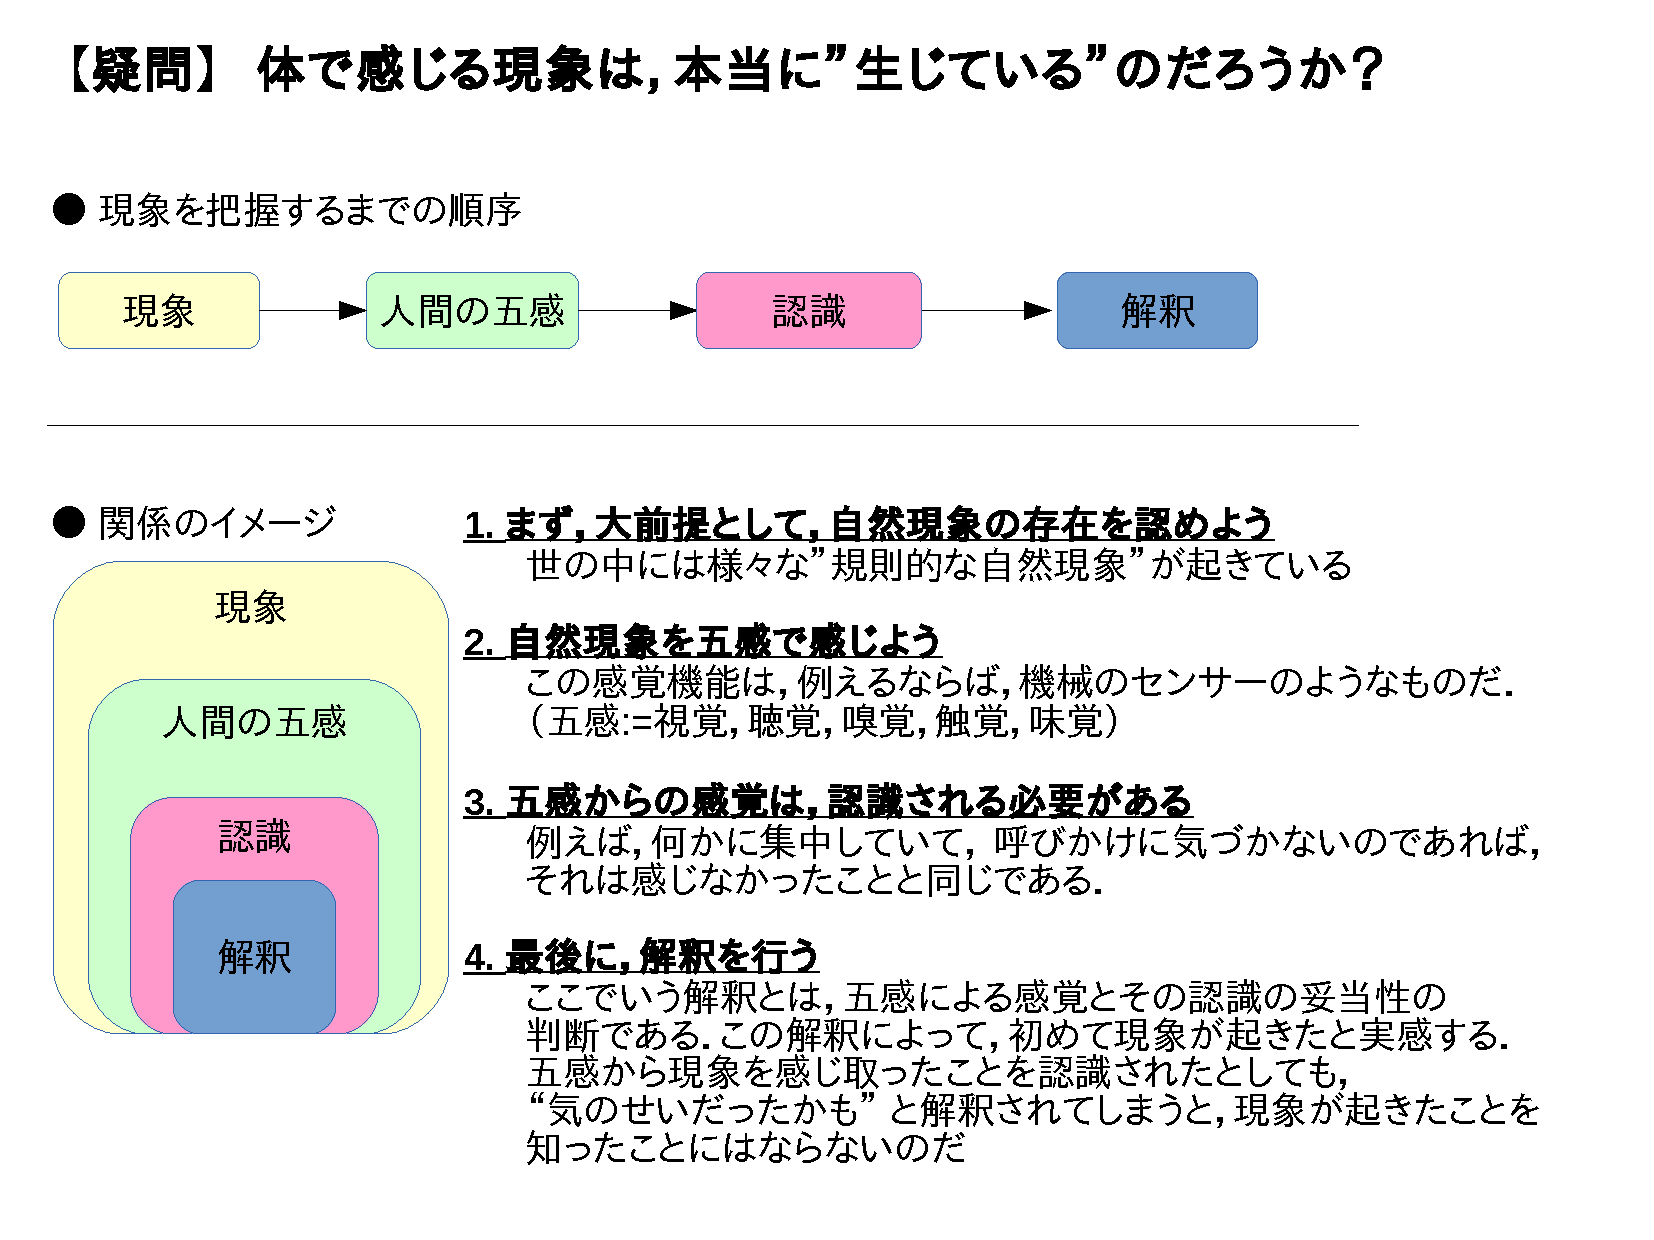
\includegraphics[keepaspectratio, width=7.2cm,height=6.35cm,clip]{kasetu.pdf}
                    \caption{科学的活動}
                    \label{fig:kasetu1}
                \end{center}
            \end{figure}

        \subsubsection{経験$=$現象を観察する}
            物理学は実験や経験を基に構成される.この経験というのは,私たちの五感
            で感じる経験のことである.この点で,経験を排除しようとする数学とは異る
                \footnote{
                    数学は,論理と算術のみによって,構成される.数学の構成には,
                    怪しげな経験などは含まれない.数学で仮定されるのは,ごく少数
                    の,それも誰もが正しいと認めるような,約束(\textbf{公理} と
                    呼ばれる)だけである.数学は,まず公理を構成し,その公理を満
                    たす対象の性質(\textbf{定理},\textbf{命題}など)を研究する.
                }.

        \subsubsection{仮説$=$現象の説明の試み}
            自然を肌で感じたことを,ノートに書き取る.いろいろ書いていくうちに,
            自然現象に共通点があることに気づく.そして,その共通点を元に,ある仮
            説をたてる.そして,その仮説を確かめるべく,実験をする.
            結果が正しければ,その仮説が立証させれたことになる
                \footnote{
                    仮説が否定さ
                    れる結果を得ることも多いが,仮説に対して肯定的な結果を得たときには,
                    さぞうれしいことだろう
                    こんな経験をしてみたい.
                }.

        \subsubsection{実験で仮説を検証する}
            何度も言うが,実験により確かめるということが重要であり,これを怠っては
            ならない.物理学の基本的な作業工程は,
            経験を元に,仮説を立て,実験をしてその仮説の正しさを確かめることである.
            立てた仮説が多くの
                \footnote{
                    「多くの」というのは,"これまで知られている法則から導出される現象よりも,
                     多くの現象が説明できる" という意味で用いた.とい言うことは,
                     古い法則が新しい法則によって上書きされるのであるが,決して古い法則が
                     間違っていたとは解釈されない.それは,法則が "拡張された" と言い訳されるのだ.
                     このへんの考え方は,おそらく物理学の学習を進めていく段階で,自ずと,身についてしまう
                     ものだ.
                }
            自然現象を説明できるのであれば,それはいつしか「法則」と呼ばれるようになる.

            実験の大まかな手順は次の通りだ.まず,仮説を検証するために妥当な実験をしないとならない.
            仮説と全く関係のない実験をしても無意味だ
                \footnote{
                    体重を測ろうとしているのに,身長を測っても仕方ないだろう.
                }.
            そのためには,\textbf{実験計画} を立てる必要がある.適切な実験方法を考えるのだ.
            そして,実験器具を揃え,注意深く実験を遂行する.実験データはノートに書き残しておく
                \footnote{
                    個人的には,紙のノートにペンで記録したい.
                }.
            実験中の異変も記録しておくべきだ.
            実験が終わったら,結果を整理し,計画通りの実験が行えたかどうかを見直す.
            間違いがなければ,これで実験の終了である.後は考察するだけだ.

            実験から統計学や論理的推論により,実験で何が得られたかを考えることを \textbf{考察} という.
            実験が終わったら,必ず考察をして,実験による得られたことを明確にすべきだ
                \footnote{
                    考察を怠るということは,実験をしなかったことにするということである.
                    実験の目的は,仮説の妥当性を実証もしくは反証することである.
                    その判断を行うための前段階として,実験結果から何が言えるかを
                    考えないとならない,
                }.
            実験結果は,多くの場合,仮説の実証や反証よりもさらに深い知識を,私たちに提供する.
            考察をすることにより,実験結果から最大限の情報を引き出すのだ.

            物理学の仮説は数学のように数と論理だけで証明することはできない.
            仮説の正しさは実験によってのみ確かめられる.実験による証明といういみで,\textbf{実証} と
            いうこともある.また,「科学的に証明された」など,科学を語る文脈で「証明」という語彙
            が使用されることも多いが,この場合の証明とは実証を意味するものである.
            「証明」とか「実証」だとかと言葉の使い方にいちいちこだわる必要はないが,
            科学的な仮説は数学のように証明できるものではないということを理解しておくべきである.

        \subsubsection{解釈(考察)$=$仮説の肯定,否定}
            さて,忘れがちなことだが,実験により得られたデータがその仮説を支持するか
            否かを判断することが必要である.このような行為を \textbf{解釈} という.
            仮説が物理法則になるための最後の関門が,この解釈である.
            多くの人々がその実験データが仮説を有力に支持すると判断したとき,
            その仮説は,法則と呼ばれるようになる.

            \subsection{自然現象の発生とその解釈}
            残念ながら,自然現象を人間が把握するには限界がある.
            いや,限界ではなく,制約という表現のほうがよいかもしれない.
            いずれにせよ,自然界で起こるすべての現象を正確に把握することは不可能
            である
                \footnote{
                    ここでは,立場を明確するために,不可能であると断言してしまったが,
                    実際のところ,こう断言するための根拠はない.主張を弱めて,
                    自然現象そのものを感じ取ることはできない,といったほうが
                    無難なのかもしれない.
                }.
            理由は,人間の五感
                \footnote{
                    「自然現象を感じ取るためのセンサー的機能」のことを指す.
                    人間が自然に対して直接的に干渉する部分は,この五感である.
                }
            と,その情報を処理する脳が絶対に正確であると言い切れないところにある.

            自然現象が発生したと人間が知る場合,まずそれは \textbf{五感} という感覚を
            通して通知される.
            そして,その感覚は脳へと渡り,初めて \textbf{認識} される.しかし,認識されるだけでは,
            まだ不安がある."気のせいだ" という判断したことがない人は,おそらく,いない
            はず.感覚を脳が認識したにもかかわらず,気のせいとしてしまい,片づけられたら,
            それは,認識されなかったことと同じである.自然現象が起きたことを確信する
            ためには,\textbf{解釈} することによる妥当性の保証が必要である.この解釈には,
            根拠ない自信であってもよいが,その現象を示す複数の感覚や証拠があるともっとよい.
            複数の人間が同じように認識したのであれば,それは有力であろう.とにかく,
            機能性ではなく,何かが絶対に起きたという解釈がなされることによって初めて,
            その現象がほんとに起こったこととして認識されるのである.

            現象を五感で感じ取り,それを脳で認識し,その妥当性を解釈によって判断することに
            よって,自然現象をとらえることができるのである.

            人間には,ウィルスを直接みることはできないし,
            超音波も聞こえず,紫外線も赤外線も見ることはできない.
            つまり,五感には限界があるということだ.
            先人はこれを克服すべく,顕微鏡を発明したり,現象を電圧や電流に変換するような
            装置を作ったりした.これによって,五感では感じ取れなかったことも"見える"ように
            なった.どうやら,五感に関する限界は,それにとってかわる装置を発明さえすれば,
            突破できるようだ.しかし,人間の思考(脳)については,今のところ,
            どんなに頑張っても,その正確性を保証することはできないようだ.

            "科学活動とは人間から見た自然現象の把握である"と考える
            人間原理的な立場では限界でも何でもないが,人間原理は
            新しい考え方を生まないために生産的ではなく,議論しても無駄だという結論しか導かれない.

        \begin{memo}{偶然と必然}
            科学では,偶然という考えは極力避けるべきである.
            自然現象は必然的に発生することであり,発生したすべての自然現象が総じて現実である.
            実際に発生していないことは必然的に発生していないのである.起きることも起きないことも
            必然であり,偶然ではない.

            しかし,必ず起きることとか,起きるかもしれないこととかの,判別の方法がない.
            偶然に起きたことだと思っていても,実はその発生は必然だったかもしれない.
            発生が必然的なものであったと思っていても,実はそれは偶然発生しただけかもしれない.

            例えば,ガラスのコップがテーブルから床へと落ちた場合を考えよう.
            仮に,コップが割れたとする.このとき,コップが割れたことは必然であろうか.
            一般的にガラスは落としたら割れるとされるので,コップが割れたことは必然であった
            とするのがしぜんであろう.しかし,もし,コップが割れなかった場合はどうか.
            コップが割れなかったことは,偶然であったと考えるのが妥当だと思うのだが,
            そう考えると,コップが割れることが必然であるという考えに矛盾する
                \footnote{
                    「落ちれば"必然"的に割れるガラスのコップが,"偶然"にもわれなかった」とは
                    どういうことか.偶然と必然は相反するものであり,
                    \textbf{必然的に起きることが偶然起きなかったなんてことは考えられない}.
                }.

            この矛盾を回避するために,可能性という概念を持ち出すことがある.
            コップが落ちたとき,コップが床に到達する直前では,コップが
            割れる場合と割れれない場合の2があるが,どちらになるかの判別は全くつかない.
            コップが床に衝突した後になってからそれがわかるのだが,割れるにせよ割れないにせよ,
            それは偶然的に起きたこととして認識される.つまり,可能性という概念を
            導入すると,現象の発生は偶然的であるということになる.だが,科学ではそうは考えない.
            床の硬度とコップの材料や形や強度とか落下速度などの必要な情報が全てそろえば,
            実際に落下しなくても,そのようなことが起きた場合を仮に想定して,割れるか割れないかの
            判別は計算によって判別することが可能であると信じるのである
                \footnote{
                    量子的な現象の場合には断定することができないのだが,
                    それでも統計的(確率的)にいうことはできる.
                }.
        \end{memo}

        \begin{memo}{相対主義と絶対主義/蓋然性の蓋然性}
            絶対に正しい真実はあるか.もしかしたら,あるかもしれない.でも,ないかもしれない.
            少なくとも,いままで見つかったことはない.答えは人それぞれであり,絶対的な答えはな
            いとする立場を \textbf{相対主義} という.他方,絶対に正しいという答えがあるとい
            う立場は \textbf{絶対主義} とよばれる.相対主義は正しいか,いや,もっと強く表現して,
            相対主義は絶対に正しいか.あれ,,相対主義が絶対に正しいとすると,絶対に正しいとする
            考えが存在するという立場にあるので,これは絶対主義である.矛盾だ.相対主義が正しいと
            主張する立場は絶対主義となる.ならば,相対主義も相対的に正しいのだと考えればどうか.
            だめだ.これでは,何も主張していないのに等しい.困った.これが相対主義のパラドクス.

            科学は仮設を実験的に検証することは可能だが,絶対に正しいとは言い切れない.
            そうかと言って,実験結果は人それぞれだというわけではないので,相対主義でもない.
            そうなると,「ある程度正しいだろう」という意味の \textbf{蓋然性} という考え方が浮上
            してくる.仮設が間違っているかもしれないという,譲歩的な気持ちがあらわれてくるのだ.
            でも,ちょっと待てよ.「『ある程度正しいだろう』という考え」はどの程度正しいのか.
            つまり,蓋然性という考え方の正しさはどの程度かI(蓋然性の蓋然性).正しさの根源を
            探ろうとすると,深みにハマる.答えが見つからない底なし沼だ.このあたりで,やめておこう.
        \end{memo}

        \begin{memo}{真偽と確実性}
            「Aであることは真実か」(真偽の問題)という質問と,「Aであることは確実か」(確実性の問題)という質問.
            両者は似ているようで異なる.真偽はあらかじめ決まっているものであり(我々が知らないだけ),実質的に根拠はいらない.
            他方で,確実性を考えるには根拠が必要である.「真であること」はありうるが,確実に真である保証はない.
            言葉と意味と論理に注意しておきたい.「『その事実が確実である』ことは確実ではない」といっているのではない.これは矛盾だ.

            例えば,未解決問題が解けたという主張があり,その主張が検証段階にある場合,
            その主張が真であるということは,確実ではない(いま,まさにこの検証をしているのだから).
            その主張が確実であるということは,真ではない(だからといって,確実でないことはない).
            確実性を問う場合には,確実ではない可能性が想定されている.真偽を問う場合には可能性は皆無である.

            真であることは真か,偽であることは真か,真であることは偽か,偽であることは偽か,真または偽であることは真か,
            同じ語彙を使う場合,メタレベルで考えないと矛盾に陥る.
            もっと,シックリくる説明はできないものか.
        \end{memo}


%       %======================================================================
%       %  SubSection
%       %======================================================================
        \subsection{論理的な飛躍}
            科学的な説明を聞いて,"もっともらしい"と感じたことはないだろうか.
            そして,それを論理的だと思ってしまったことはないだろうか.
            しかし,この感覚は間違っている.科学は論理的ではないのである.
            確かに,論証は論理的であるが,科学の根源的な法則は,論理的に導かれたものではない.
            先に説明したように,科学法則は経験や実験から推察することによって,
            得ているものであることを忘れてはいけない.この推察の部分に論理的飛躍があるのだ.

            \begin{memo}{例:ハッブルの法則}
                しばしば,仮説を表す命題の前提と結論を逆にすることにより一般化し,
                法則として捉えなおされることがある.

                具体的な例で考えてみよう.「ハッブルの法則」と言われている法則がある
                    \footnote{
                        ハッブル [著],戎崎 俊一 [訳],『銀河の世界』,岩波文庫
                    }.
                この法則が示すのは,宇宙が膨張していることである.その根拠は実験(観測)結果
                による.地球から見える天体が,遠ざかる速さとその距離が正比例する,というのが
                実験事実である.そして,そこから,宇宙が膨張していることが示されるという.
                論旨を追ってみると,まず,天体同士の距離が時間が経つごとに開くという観測事実
                がある.この現象は地球から見える宇宙のどの方向でも例外なく起こっていて,天体
                が近づくことはないという.つまり,宇宙のある所では天体間の距離が小さくなりつ
                つあり,別の所ではその距離が開きつつあるというのではなく,宇宙のいたるところ
                で,天体間の距離が同じように開いているというのである.宇宙の広がりに関する状
                態として考えられるのは3種類あり,
                (1)静止状態
                    \footnote{
                        広がったり縮まったりしておらずに定常状態を保っている,ということ.
                    },
                (2)広がりつつある状態,(3)縮まりつつある状態,である.
                この宇宙の3つの状態のうちでハッブルの法則に矛盾しないのは,(2)広がりつつある
                状態である.さらに,天体間には重力という引力が働いているので,天体同士が反発
                するということはありえない.つまり,宇宙は膨張していると結論できる,という.
                以上の論旨を整理しよう.
                    \begin{enumerate}
                        \item 天体間の距離は,宇宙の至る所で,広がりつつある(前提1$=$観測事実)
                        \item 天体同士は重力が働いていて,斥力はない(前提2$=$観測事実)
                        \item 宇宙が膨張しているとしないと,矛盾が生じる(論理的整合性の考慮)
                        \item だから,宇宙は膨張している(結論)
                    \end{enumerate}
                前提が実験事実である天体間の距離の拡大であり,結論が
                宇宙の膨張であるということに注意してほしい.ここまでは論理的な推論である.

                しかし,科学的解釈を加えると,ここから話が飛躍する.天体間の距離の拡大と宇宙
                の膨張を比べると,宇宙の膨張の方が根源的事実であり,天体間の距離の拡大は宇宙
                が膨張していることにより生じる1つの現象である,と考えるのが妥当だろう.要す
                るに,天体間の距離が広がりつつあるのは宇宙が膨張しているからである,という命
                題が立てられるのである.この命題は,さっきの論旨の逆である.以下のように記号
                化してみよう.
                \begin{description}
                    \item[A:] 天体間の距離は,宇宙の至る所で,広がりつつある
                    \item[B:] 宇宙は膨張している
                \end{description}
                法則を探り当てた段階では,A$\rightarrow$B だったが,一度宇宙の膨張が導かれる
                と,B$\rightarrow$A に置き換えられてしまった.論理的には,逆は必ずしも真には
                ならないのに.

                ここからは,B$\rightarrow$Aを法則として捉えてみよう.事実として現実に現れて
                いるのは,Aの天体間の距離の拡大である.そしてその根拠として,Bの宇宙の膨張が
                主張されている.しかし,この論理(B$\rightarrow$A)からは,AからBを導くことは
                できない.BはAを引き起こすことのできる1つの現象であると言えるが,それが唯一
                であるとは限らない.実際は何か別の現象Cがあって,C$\rightarrow$Aが成立してい
                ることも可能性として考えられるのだ.しかし,現在Cという可能性は提唱されてお
                らず,B$\rightarrow$Aの妥当性が極めて高いため,これを法則といっているのだ
                    \footnote{
                        論理的には,AとB$\rightarrow$Aが与えられた場合,"Bの可能性がある" としか
                        言えない.AとB$\rightarrow$Aから.これを科学法則に仕立てあげるには,
                        B以外の原因Cが起こり得ない(現実的に考えにくい/起こりにくい)ことを
                        示さなければならない.
                    }.

                科学的推論は論理的ではない.頻繁に使われる帰納的推論やアブダクションは必ずしも正しい結論に到達
                するわけではない.また,意図的に前件否定,後件肯定などが行われる.だから,科学には実験的検証と
                いう作業が欠かせない.科学には実験がつきものである理由がここにある.そして数学との違いも,ここ
                にある.

                数学的推論は,人間のうっかりミスなどがない限り,必ず正しい結論に到達する.ABC予想」,
                「リーマン予想」など予想があるが,これらは証明されていないので,「予想」とされている.
                科学であれば,現状観測し得るすべての場合で,その予想に反する事実がなければ,「正しい」
                とされる.しかし,数学は論理的推論によりその結論に達しない限りは,正しいとみなされない
                    \footnote{
                        数学は科学ではない.数学は科学の最重要な道具であるが,科学ではない.数学の方が
                        論理的に厳密である.数学は現実を反映しない.現実を離れて抽象化される.現に,物
                        理学的には,この世界は空間3次元と時間1次元の世界であるが,数学では次元は無限に
                        さえなり得る,科学は世界に忠実であろうとするが推論や論理に穴がある.数学は誤り
                        はないが,必ずしも現実世界に忠実であるとは限らない(現実を離れた抽象化できる).
                    }.
            \end{memo}

%       %======================================================================
%       %  SubSection
%       %======================================================================
        \subsection{推論の種類}
            科学は,実際の現象を感じ,その規則性を推論し,仮説を立てて,実験により
            その仮説を検証してその正しさを確かめることで,知識を増やしていく.
            その過程で行われる推論は大きく分けて3つある.ここで,推論という行為
            について,少し考えておこう.一言で推論といっても,その方法はいくつも
            ある.しかし,共通して言えることは,すでに得られている知識から,新しい
            知識を導き出すことである.その方法は,
            \textbf{演繹的推論},\textbf{帰納的推論},\textbf{発展的推論} がある.

%           %==================================================================
%           %  SubsubSection
%           %==================================================================
            \subsubsection{演繹的推論}
            演繹的推論は,例えば,数学の定理証明で使われる推論であり,三段論法を
            駆使して行われる行為である.この演繹的推論では常に正しい結論を得ることが
            できる
                \footnote{
                    もちろん,ケアレスミスなどの,人的な誤りがなければ,という
                    ことだ.人的な誤りはミスは必ず見つけれる.
                }.

%           %==================================================================
%           %  SubsubSection
%           %==================================================================
            \subsubsection{帰納的推論}
            帰納的推論とは,いくつかの現象から共通な部分を抜き出し,
            法則性を導き出す行為である.例えば,ケプラーの天体の運動に関する3つの法則
            は,帰納的推論により導き出されたものである.膨大な天体観測記録から,
            天体の運動の仕方に規則性を見出したのである.

%           %==================================================================
%           %  SubsubSection
%           %==================================================================
            \subsubsection{発想的推論}
            発想的推論とは,過去の経験や知識を基に,因果関係を探る行為である.
            例えば,ニュートンが発見した万有引力は,発想的推論により導き出された
            ものである.手で持った物体を,ある高さから静かに手を放すと,地面に
            落ちる,という現象が目の前で起こっているとする.物体が落ちるという現象は
            見ることができる明らかな事実であるが,その落ちる原因は直感的にはわからない.
            なので,推論によってその原因を探る必要がある.ものが落ちるという現象を引き起こす,
            もっともらしい原因を見つけ出す行為こそが,発想的推論なのだ.形式的に言えば,
            現象Xが知られていて,その原因として,仮説Yが成立していれば,現象Xが起こること
            が必然だとすると
                \footnote{
                    今までの例で言うと,X:物体の落下,Y:万有引力の法則 となる.
                },
            仮説Yが成立しているという結論が有力に支持される.もちろん,現象Xを
            説明できるのは,複数の仮説が考えられるはずである.この複数の仮説から
            真の原因を選び出すためには,実験と推論を繰り返す必要がある.
            発想的推論を短くいうならば,"Xであるという事実" を目にしたとき,
            "YならばXであるという必然的因果関係" があるならば,"Yかもしれない" という
            結論を得る推論ということになる.

%           %==================================================================
%           %  SubsubSection
%           %==================================================================
            \subsubsection{科学的推論}
            \begin{mysmallsec}{長所と短所}
            帰納的推論と発想的推論の長所は,新しい知識を生み出すことができるところだ.
            欠点は,人の経験や思いつきなどが絡みあい,
            間違った結論を導き出すという危険な副作用があるということ.
            更に欠点をいうと,これらの推論で得た結論は,将来起きる未知なる現象により,
            覆される可能性があるということだ.実際に起きていないことや過去に経験のないことに対しては,
            何も手が出せないのである.

            これに対し,演繹的推論は常に正しい結論を導くことはできるが,
            新しい知識を作り出すことはできない.しかしその代わりに,一度導き出された
            知識は,未来永劫にわたって真であり,覆される可能性は全くない.
            \end{mysmallsec}

            \begin{mysmallsec}{科学的推論}
            科学と数学と違いは,帰納的推論と発想的推論にある.
            これらの推論には間違いが含まれるかもしれないというリスクはあるが,
            それを補ってあまりある新しい知識を創造できるのである.
            対して,数学は演繹的推論のみを採用しており,帰納的推論と発想的推論は
            禁止されている.それが故に,数学はいつなん時でも正しい結論が得られる.

            科学的推論とは,帰納的推論や発想的推論で得られた知識を,
            演繹的推論によって洗練させて,実際に起来ている(あるはこれから起きるだろう)
            現象に対する有力な説明を与えることである.
            \end{mysmallsec}

%       %======================================================================
%       %  SubSection
%       %======================================================================
        \subsection{再現性}
            経験より得られた仮説は,実験を行って,その正しさを確かめないといけな
            い.けれど,全ての仮説に対して,実験が行えるわけではない.実験不可能
            な仮説も存在するのである.

            実験不可能な仮説の有名な例として,「幽霊の存在」がある.なぜ,幽霊の
            存在を実験的に確かめることができないのだろうか.ここには,実験の再現
            性がかかわっている.

            実験に要求されることのひとつとして,再現性がある.\textbf{再現性} と
            は,同じ環境で同じように実験を行うと,同じ結果を得ることだ.全く同じ
            条件で,全く同じ方法で実験を何回か行って,それぞれで異なった結果を得
            るのでは意味がない.もし,毎回結果が異なるのであれば,検証すべき
            その仮説は間違いであったと結論されるか,実験が正しく行われなかったか,
            原因は様々であるが,いずれにしても,何も得られなかったことになる.

            幽霊の存在の話に戻ろう.幽霊が存在することを実証できないのも,
            再現性のある実験方法がわからないからである.突如として現れる幽霊は,
            その発生条件すらもわからず,おまけに,目で見えたり見えなかったりする.
            心霊写真といわれるものがあるらしいが,それも幽霊の存在の実証にはなら
            ない.こうすれば絶対に幽霊の写る写真が取れる,という方法が確立されれ
            ばよいが,成功例はなく,難しいようである.

            再現性が要求されるのは,誰でも確かめられるということが重要だからであ
            る.客観的に自然現象を捉えるには,再現性は非常に重要な要請である.

            実をいうと,現在の物理学の実験は多くの場合非常に難しい実験であり,何
            度でも誰でも気軽に行えるものではない.それでは再現性があるとはいえな
            いのではないか,と考えてしまうかもしれないが,物理学者は再現性をもっ
            と緩くとらえているようである.すなわち,物理学者は,再現性がある実験
            かどうかを判断し,再現性があるだろうことが認められれば,それで良し
            とするのである.このことについて,中谷宇吉郎
                \footnote{
                    中谷宇吉郎(1900--1962, 日本):物理学者.雪についての研究が
                    一般的に有名.「雪は天から送られた手紙である」という有名な文
                    句でも知られる.
                }
            の易しい説明があるので,これを次に引用しておこう.
                \begin{memo}{「科学の方法」(中谷宇吉郎:岩波新書)より}
                    科学について,何かを論じようとする場合に,まず取り上げるべき
                    問題は,科学の限界の問題である.今日われわれが科学と称してい
                    るものは,その取り扱い得る問題,限界があるか否かというを,ま
                    ず検討してみる必要がある.

                    今世紀(20 世紀) に入って,科学が非常に進歩し,特に自然科学が
                    最近になって,急激な発展をとげたことは,いまさら言うまでも
                    ない.いわゆる,人工頭脳のような機械ができたり,原子力が解放
                    されたり,人工衛星が飛んだりしたために,まさに科学ブームの世
                    の中になった観がある.そしてこの調子で科学が進歩を続けていく
                    と,近い将来に人間のあらゆる問題が,科学によって解決されるで
                    あろう,という異様な錯覚に陥る人が,かなりあるように思われる.

                    もちろん科学は,非常に力強いものではあるが,科学が力強いとい
                    うことは,ある限界の中での話であって,その限界の外では,案外
                    無力なものであることを,つい忘れがちになっている.いわゆる,
                    科学万能的なものの考え方が,この頃の風潮になっているが,それ
                    には,科学の成果に幻惑されている点が,かなりあるように思われ
                    る.これは何も人生問題というような高尚な話ではなく,自然現象
                    においても,必ずしも全ての問題が,科学で解決できるとは限らな
                    いのである.今日の科学の進歩は,いろいろな自然現象の中から,
                    今日の科学に適した問題を抜き出して,それを解決していると見た
                    ほうが妥当である.もっとくわしくいえば,現代の科学の方法が,
                    その実態を調べるのに非常に有効であるもの,すなわち自然現象の
                    中のそういう特殊な面が,科学によって開発されているのである.

                    それはどういう面かというに,まず第一に,一番重要な点をあげれ
                    ば,科学は再現可能な問題,英語でリプロデューシブルといわれて
                    いる問題が,その対象となっている.もう一度繰り返して,やって
                    みることができるという,そういう問題についてのみ,科学は成り
                    立つものである.

                    なぜ再現可能の問題だけしか,科学は取り扱い得ないかといえば,
                    科学というものは,あることをいう場合に,それがほんとうか,ほ
                    んとうでないかということをいう学問である.それが美しいとか,
                    善いとか悪いとかということは,決していわないし,またいうこと
                    もできないものである.

                    それでは科学で,ほんとうであるというのは,どういうことかとい
                    うことを,まず考えてみる必要がある.ごく簡単な場合についてい
                    えば,いろいろな人間が同じことを調べてみて,それがいつでも同
                    じ結果になる場合には,それをほんとうというのである.最も
                    同じことを同じ方法で調べることができない場合もある.しかし人
                    間が自然界を見るときには,いつでも人間の感覚を通じてみるわけ
                    だが,この感覚を通じて自然界を見ることによって,ある知識を得
                    る.その得た知識と,他の人がその人の感覚を通じて得た知識と
                    の間に,互いに矛盾が無い場合には,われわれはそれをほんとうで
                    あるという.そうでない場合には,それはまちがっているというわ
                    けである.

                    (中谷宇吉郎[著],『科学の方法』,岩波書店(岩波新書),1998 より
                    \footnote{
                        初版は1958年.
                    }.)
                \end{memo}


%       %======================================================================
%       %  SubSection
%       %======================================================================
        \subsection{単純性:オッカムの剃刀}
            理論はできるだけ複雑にならないように組み立てるべきだ.
            この考え方を,\textbf{オッカムの剃刀} という
                \footnote{
                    William of Ockham(13世紀後半--14世紀前半,イギリス):
                    英語表記をそのまま訳すと,「オッカムのウィリアム」となる.
                    「オッカム」というのは,当時のイギリスの地名.
                    ウィリアムという名前でなく,地名であるオッカム
                    のみがその表現に残っているのかは不明.
                }.
            何かを説明するのに,必要以上の仮定を避けるべきだ,という考え方
            である.必要以上の仮定が含まれている理論を,カミソリによってそぎ落とし,
            より単純化するイメージ.

            但し,初めて人に説明するときは,これを正直に実行してしまうと,
            簡潔すぎて正しく伝わらないことだろう.
            概念をわかりやすく説明するためには,初めは多少遠回りをして,物事を考えるこ
            とも必要である.その場合,概念を理解した後に,単純性を満たすよう
            に整理すればよい.

            そうかといって,最も単純な理論がどのようなものなのかはわかりよう
            もない.単純さという感覚はどうにも曖昧だからだ.つまり,これには
            答えがない.「おぉ,単純だ.美しい!!」という直感が大事だ.

            もちろん,最初からできるはずもない.最初は何もわかっていないのだ
            から,論理的に不完全な推論しかできない.しかし,その推論がどうも
            正しい方向にあると感じたら,その足りない部分を補って,理論を構成
            していく.理論を構成していく上で,それまでに必要だと思っていたこ
            とが,実際には無駄なことであったというような部分も,見つかるかも
            しれない.そうした無駄な部分は削除される.こうして,単純な理論が
            構築されていく.時間をかけて無駄な部分を省き,シンプルにしていく
            のだ.

            単純性を追求してしまうと,それと同時に,「理論を作り上げるまでの
            考え方」も,削除されてしまう.どのようにして,その理論を作り上げ
            たのかが,わからなくなってしまうのである.いま学習している物理学
            は,既に単純化された理論である.この単純化された理論は,初めて物
            理学を学習する場合,とてもとっつきにくいものになっているだろう.
            なぜなら,単純な理論を構築するときに,その構築方法までも削除され
            ているからだ.理論を受け入れる場合は,単純な理論ではなく,理論に
            無駄部分はあっても,受け入れやすい形であることも大事である.理論
            の受け入れ方として,まず無駄な部分を含むが受け入れやすい形で,そ
            れを理解し,その後に単純化された理論を再度学ぶという方法がよい.

            ちなみに,このように,できるだけ理論を単純化しようとする動き
            を \textbf{思考経済} とよんだりする
                \footnote{
                    オッカムの剃刀と同じことを主張する,別の言い方.
                    いろんな言われ方があるくらいに,重要な考え方なのだ.

                    Everything should be made as simple as possible, but not simpler.
                    (A. アインシュタイン)
                }.
            できるだけシンプルに考える
            という思考方法である.思考経済は物理学に限ったことでなく,学問
            であるならば必ず採用されて いる.学問体系を構成する理論が冗長で
            あっては格好が悪いし,できる だけシンプルにまとまっていた方がわ
            かりやすいのだから.

            \begin{memo}{「オッカムの剃刀」は正しいのか}
                オッカムの剃刀は全面的に正しいとは限らない.
                単純な理論ほど良い理論であると,必ずしも言えないのだ.
                最も単純な理論は,神を持ち出すことである.
                どんな複雑な現象でも,神を理由にすれば,その説明はとても単純になる.
                少なくとも,いま知られている
                物理法則から現象を説明するよりは単純になる.しかし,これでは本末転倒だ.
                物理学の目標は,神を持ちださないで物理現象を説明することなのだから.
                つまり,オッカムの剃刀という考え方にも,適用限界があるということだ.
                どこに限界があるかを考えるべきだが,簡単には答えは見つかりそうもない.
                とても難しい.

                ここでは,オッカムの剃刀と言う考え方は不完全であることを
                気に留めておくことにし,難しい議論は避けよう.
            \end{memo}


%       %======================================================================
%       %  SubSection
%       %======================================================================
        \subsection{客観と主観}
%           %==================================================================
%           %  SubsubSection
%           %==================================================================
            \subsubsection{客観性}
                物理は客観的であるべきだ.しかし,物理学は本当に客観的に構成されているのだろうか.
                物理学に要求される客観性とは,どういったものなのだろうか.
                ここで,少し考えてみたい.

                世の中に存在するヒトの人数は,数十億人と
                言われる.物理で扱われる事柄は,これら数十億人のヒトにとって,
                共通でなければならない.言い換えれば,解釈がヒトによって異なってはならない.
                この客観性が,物理に課せられた条件の1つである.

                しかし,実際のところ,物理学を少し学習していくと,あるいは,
                物理学の啓蒙書を読みあさってみると,物理の解釈が人それぞれで異なって
                いるように,感じられる
                    \footnote{
                        「物理の」と曖昧に書いている.具体的には,「物理法則の」と
                        読み替えてもらえると,話が通じるはず.
                    }.
                つまり,物理は,完全には客観的では
                ないということである.おそらくこれは,物理が経験に基づいていることにあると思う.

                物理は数学とは違い,人間の経験を基に
                理論構築される.その理論の正しさの確認も,実験という経験を
                通してなされるものである.もちろん,経験といっても,一人の人間しか
                経験できないようなものではなく,すべての人ができる経験である.

                物理学に課せられている客観性とは,全ての人が経験できる事柄である.
                そして,その経験はすべての人に共通でないといけない.しかし,経験は
                人間ひとりひとりが感じるものであり,その感じ方(解釈)は人によって
                ことなる.だから,物理学ではこのような解釈の違いを排除すべく,
                基本単位を定義することにより,客観性を作り上げている.
                例えば,温度などは,"熱い"や"冷たい"などと表現するのではなく,
                セ氏何度という表現をしている.温度計を用いて,温度を測定する事により,
                熱いや冷たいなどと表現するのではなく,「セ氏20度」などと,万人に
                共通であるようにしているのだ.これにより,温度が客観的に表現された
                ということになる.

                もう少し,温度の例を考え続けよう.よく考えてみると,客観的に表された
                と思った温度であるが,本当に客観的なのだろうか.ここでいう「客観的」という
                語彙の意味は,すべての人にとって,同じであるという意味である.
                つまり,「セ氏20度」はすべての人に共通なのだろうか.共通であれば,
                客観的であるといえよう.しかし,それを知る術はないし,さらに言えば,そうではありえない.
                なぜなら "「セ氏20度」はすべての人に共通" ということは,「セ氏20度」という温度を
                経験する全ての人が,全く同じように暖かさを感じるということになるからである.
                これは,今までの私達の経験に反している.北海道などの北部に住む人々にとって,
                セ氏20度は,暖かく感じられ,沖縄などの南部の地方に住む人々にとっては,涼しく
                感じられるのではないか.更に言うと,一人の人間でも,季節の違いにより,温度の
                感じられれ方はことなる.夏のセ氏20度は涼しく感じられるし
                    \footnote{
                        むしろ寒いくらいだ.
                    },
                冬であれば暖かく感じる.セ氏温度により,客観的に温度を表現はできるものの,
                温度を感じるのは人間であり,つまり,そこに主観が入り込んできて,客観性が
                失われる.では,「セ氏温度の導入が,物理に客観性を生むのに失敗しているのだろうか」といえば,
                それは違う.現に,温度計を用いて温度を測ることには,客観性があることは,
                明らかである.いつでもどこでも,セ氏20度が変わることはない.

                ここに,温度の客観性に関して,矛盾が感じられる.大げさに言えば,
                宇宙のどこで測っても,セシ温度は共通であり,つまり,温度が客観的に
                表現されている.一方で,温度とは,人間が感じるものであり,その感じ方は,
                人それぞれ違うものであり,また,時期によってもその感じられ方は異なるので,
                客観性がないように思われる.どこが間違っているのだろうか.答えは簡単で,
                人それぞれの感じる温度を客観的に示すべくセ氏温度が導入されたのだから,
                温度を感じる人間を持ち出したことが,間違いであったのだ.要するに,人間の体験
                の排除をすることにより,客観性を産み出しているのである.セ氏20度の
                感じ方は,人それぞれ違うのは当たり前.それを統一すべくセ氏温度が導入されたのだ.

                別の例を上げてみよう.色に関する経験を考えてみる.「青」という色は,
                全ての人間に全く同じように感じられるのだろうか.答えはあからかにNoである.
                「青」という色を感じ取るのは,人であり,個体差があって当然である
                    \footnote{
                        目の作り,目で感じた光を脳に伝える神経の作り,脳の作りなど,
                        色を感じるための機構が同じである二人以上の人間がいるとは考えにくい.
                        色の感じ方は,人によって違うと考えたほうが自然である.
                        まあ,人によって同じかどうかということを考えることそのものが,
                        無意味である.なぜなら,確認のしようがないのだから.
                    }.
                では,物理では色を客観的に示すことはできないのだろうか.もちろん,そんなことはない.
                色は光であり,光は電磁波という波の一種であることがわかっている.物理で言う色の違い
                とは,この波の波長
                    \footnote{
                        周波数といっても同じことだ.$\nu T = 1$ ($\nu$ は波の周波数,$T$ は波の周期) の
                        関係式が成立しているはずである.周波数とは,一秒間で振動する波の回数であり,
                        周期とは,一回の振動にかかる時間のことである.つまり,$T = 1/\nu$ が成り立つ.
                        一秒間に $\nu$ 回振動するのだから,1を $\nu$ で割ることにより,周期を計算できる.
                    }
                の違いである.色を波長という数値で定義することができ,これにより,人間の
                体験の排除が実現されるのである.色を感じるのは確かに人間であるが,色を客観的に
                表現するには,人間の経験を排除しなければならない.その代わりに,番人に共通である
                波の波長という数値を導入するのである.

                長々と書いてしまったが,話を元に戻そう.何が言いたかったかというと,
                物理学における客観性とは何かということである.その答えは,もう既に
                書いてしまったが,\textbf{人間の体験の排除}である.数値は万人にたいして
                客観的事実を伝えるのであるから,人間の体験を数値で置き換えることをすることにより,
                客観性を保とうとしているのである.

%           %==================================================================
%           %  SubsubSection
%           %==================================================================
            \subsubsection{"客観" と "主観" の違い}
                物理,あるいはもっと範囲を広げて,科学とは客観的に構成される.
                しかし,客観的な科学はそのままでは,使いものにはならない
                    \footnote{
                        物理法則の理論的な側面だけを追求しようとする人には,
                        それで十分だと思われるかもしれないが,それにしても,
                        その物理法則の捉え方は人それぞれ解釈が異なる.
                        (式の解釈が万人に共通であるとは考えにくい.法則を表す式は一般的に
                        表現されるものであり,完全に意味付けされていない.具体的に意味づけしようと
                        する際に,解釈の違いが生まれてくる.これから,学習するニュートンの法則
                        もそれに同じ.図書館などで多くの教科書を探ってみよう.様々な説明のされ方が
                        なされることを知るだろう.)
                    }.
                科学は解釈しなければ,使うことができない.解釈するということは,そこに
                解釈者の主観が交じるということである.
                この解釈するという行為は,勘違いしやすく,矛盾に陥りやすい
                ところなので,特に注意しないといけない.

                科学を解釈するということは,客観的に記述されている科学的事実を解釈するという
                ことであり,科学が客観的でなくなるわけではない.

                科学の理論構築は,始めは人間の経験や体験によるものであるが,それを
                数値化することで,客観性をつくり出している.科学理論は客観的
                である.それを解釈するのは人間であり,この時に科学の客観性が失われ,主観が生じる.

                科学のおける客観性と,その解釈により生じる主観性は区別して考えなければならない.

%           \begin{memo}{「数」と「量」}
%               モノの個数を数えることを考えよう.具体的に考えるため,モノの例に果物をとる.
%               目の前に,林檎,蜜柑,苺,葡萄,桃がそれぞれ置かれているとしよう
%               (図\ref{fig:kudamono})
%                   \footnote{
%                       とりあえず,5種類を上げたが,この説明で使用するのは林檎と蜜柑
%                       だけ.他の果物は特に意味のないもの.果物がたくさんあったほうが,
%                       見栄えがいいでしょ?
%                   }.
%                   \begin{figure}[hbt]
%                       \begin{center}
%                           \includegraphicsdouble{kudamono.pdf}
%                           \caption{目の前に,美味しそうな果物が!}
%                           \label{fig:kudamono}
%                       \end{center}
%                   \end{figure}
%
%               それぞれの果物の個数は,見るからに異なる.では,どれだけ違うのか.
%               直接示して,林檎は
%                   \begin{figure}[hbt]
%                       \begin{center}
%                           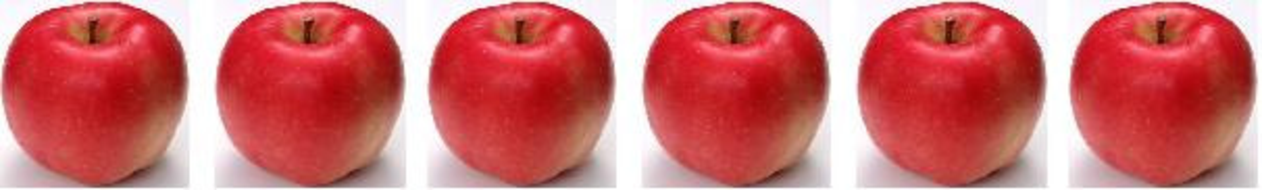
\includegraphics[keepaspectratio, width=3cm,height=0.5cm,clip]{kudamono_apple.pdf}
%                           \label{fig:kudamono_apple}
%                       \end{center}
%                   \end{figure}
%               であり,蜜柑は
%                   \begin{figure}[hbt]
%                       \begin{center}
%                           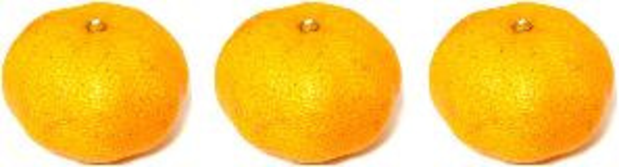
\includegraphics[keepaspectratio, width=1.5cm,height=0.4cm,clip]{kudamono_orange.pdf}
%                           \label{fig:kudamono_orange}
%                       \end{center}
%                   \end{figure}
%               だ,といったところで,具体的な個数の違いを示せない.
%
%               ここで,\textbf{数} という概念が有用になる.\textbf{一対一対応} という考え方を使うのだ.
%                   \begin{figure}[hbt]
%                       \begin{center}
%                           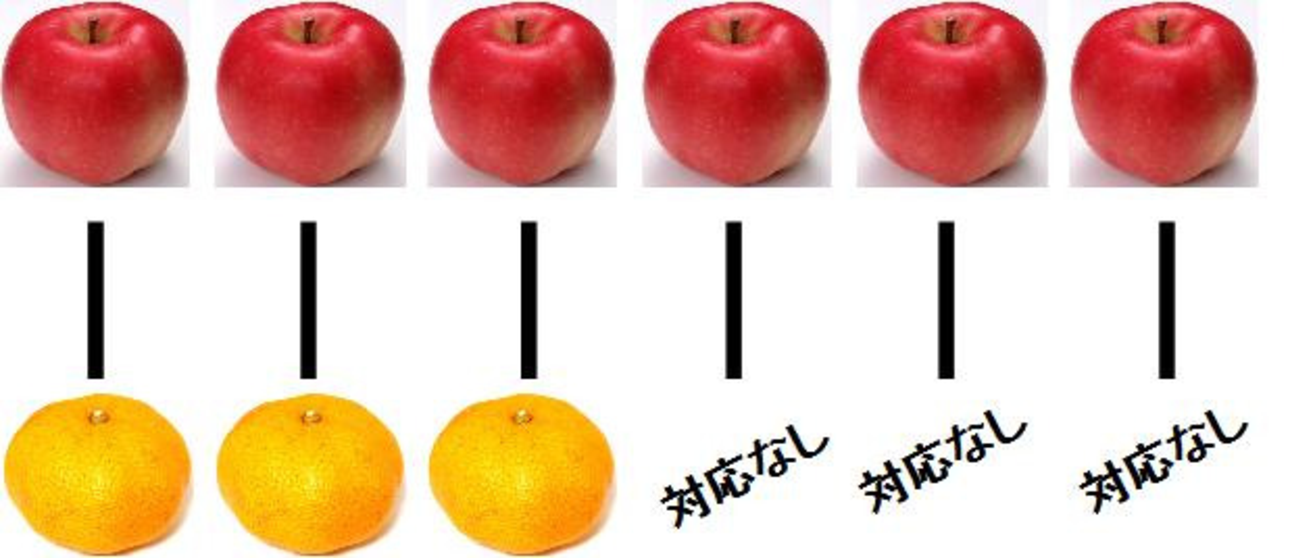
\includegraphics[keepaspectratio, width=4cm,height=1.8cm,clip]{kudamono_comp.pdf}
%                           \label{fig:kudamono_comp}
%                       \end{center}
%                   \end{figure}
%           \end{memo}

%       %======================================================================
%       %  SubSection
%       %======================================================================
        \subsection{法則}
%           %==================================================================
%           %  SubsubSection
%           %==================================================================
            \subsubsection{還元主義}
            科学は \textbf{還元主義} という思想が強く反映されている.
            還元主義とは,どんなに複雑に見える現象でも,それらを詳細に分析
            することで,複数の簡単な問題に捉えなおすことができる,という
            考え方だ.

            物理学の目的の1つに,「少数の規則を議論の出発点として,現実に起こっている
            現象を説明すること」というものがある.しかし,実際の全ての現象が,
            少数の規則
                \footnote{
                    少数の規則:"少数"と曖昧に表現したのは,
                    個数には特にこだわらないからである.
                    しかし,規則の個数は有限個である必要があることを要求する.
                }
            で説明できるという保証はない.人がそう信じているだけだ.
            しかし実際のところ,この考え方によって物理学は発展している.
            もちろん,説明できない現象も多いが,それらについても,
            将来の物理学の発展によって,説明可能であるとされている.
            要するに,何の根拠もない考え方だけど,今までこの考え方で成功してきているのだ.

            還元主義は,今まで大成功を収めているので,根拠がないという理由で捨てることは
            できない(もったいない).足元が不安定に感じるかもしれないが,
            信じるしかないようだ.

            \begin{memo}{科学的思想の根本?}
                還元主義に根拠がないなど,科学の思想的土台はとても不安定だ.
                そもそも経験に根拠があるはずがなく,それ基にした学問だから仕方ない.
                科学とは,多くの人間の様々な経験の中から,"いつもそうなる" というものを抜き出して,
                それらを整理して体系立てることである
                    \footnote{
                        いろんなところで,"科学とは" といった説明を聞くだろう.
                        実際,このノートでも複数の箇所に,そういった表現がある.
                        しかし,そこで表現されていることが唯一ではなく,
                        科学という活動にはそういった一面もある,ということを言いたい.
                    }.
                科学に対して,論理学や数学のような強い理論的土台を求めてはならない.
                間違いに気が付いたら見直す,というくらいの気構えが必要だ.

                こう言ってしまうと,「科学的に立証された」という表現に対して,
                少々不信感が出てきてしまうかもしれない.それは正しい.科学には
                潜在的な間違いが含まれていることを,承知しておくべきだ.
                しかし,だからと言って,科学を過渡に拒否するのはもったいない.
                先人の多くの経験や実験による成果によって,現在の科学技術を駆使した
                生活があることも事実である.

                科学は間違っている部分もあるけれど,だからと言って,それを捨てるのは
                得策ではない.もし,間違っているかもしれないと感じた部分があれば,
                それを確かめるための実験を繰り返し行うことで,信頼性を高めることが
                可能だ.科学を安易に信頼するのも,過渡に拒絶するのもよくない.
                科学の性質を理解して,適切な認識をもつことが理想である.
            \end{memo}

%           %==================================================================
%           %  SubsubSection
%           %==================================================================
            \subsubsection{規則性の発見}
            実験や経験を基にして物理学を構成するには,まず,それらを言葉で表現す
            る必要がある.例えば,「落とした消しゴムは,拾わないと机には戻らな
            い」とか,「破れた紙は,元の状態に戻すことはできない」とかといった
            具合に.ときには,数式で表現されることもある
                \footnote{
                    数式によって表現されても,その根底には,言葉による表現がある.
                    言い換えれば,言葉による表現を数式として表すということだ.物
                    理は記号の羅列ではない.あくまでも,肌で感じた経験と,実験で得
                    た知識を前提にして,物理学は構成される.
                }.

            いろいろと,経験・実験を繰り替えしていき,それを言葉によって書き留め
            る.多くを経験したり,多くの実験を行えば,書き留められる言葉もそれだ
            け多くなる.このたくさんの言葉による経験・実験の記述を読み返し,吟味
            してみると,何かそれらの間で共通する部分を見出すことになる.

            例えば,「『鉛筆』は机の上から床に落ちる.拾わないと机の上には戻らな
            い」と言う記述と,「『教科書』は机の上から床に落ちる.拾わないと机の
            上には戻らない」という記述があったとしよう.鉛筆だろうが教科書だろう
            が,落ちたものは拾わないと元の位置には戻らない.当たり前のことだが,
            このことに気づくことが大事である.これが「法則」を得る第一歩だからで
            ある.

            ニュートン
                \footnote{
                    Sir Isaac Newton(1643--1727, イギリス):物理学の創始者.ケ
                    プラー(Johannes Kepler, 1571--1630, ドイツ)が唱えた「天体の
                    運動の3つの法則」を含む,物体の運動に関する3つの法則を提唱し
                    た.天体の運動と,地上ある「もの」の運動を同一視(同じように
                    見るということ)し,力学(「ニュートン力学」)を作り上げたの
                    である.「Philosophiae Naturalis Principia Mathematica」(和
                    訳名:自然哲学の数学的諸原理,もしくは,プリンキピア)によっ
                    て,現在に伝わっている.この過程で,微積分学を生み出した.数
                    学においても大きな貢献があるのだ.二項定理の証明も行っている.
                    また,物理学の他の貢献として,冷却の法則や光学に関する考察も
                    有名である.
                }
            は,たった3つの記述によって,どんな「もの」運動でも記述できることを示
            した.このような3つの記述のことを \textbf{法則} という.法則とは,ど
            んな「もの」でも,もっている性質である.

            規則を発見したところで,これからもその規則が成り立つという保証はどこにも
            ない.これを補うためには,反例を立証できないとあきらめの雰囲気が出るくらい,
            何回も実験を繰り返すことしかできない.

%           %==================================================================
%           %  SubsubSection
%           %==================================================================
            \subsubsection{法則は理論の土台である}
            物理学にはいくつかの \textbf{法則} がある.法則とは,実験によって確認される現象である.
            法則は論理的に説明されるものでもなければ,他の概念から定義されるものでもない.
            法則は理論の最も基本的な土台であり,実験のみによって実証されるべき仮説である.
            「なぜ法則が成り立つのか」を考えること は大事なことだが,それはとても難しい問題
                \footnote{
                    「難しい問題」とは,「解くのにものすごく時間がかかる」という意味であり,
                    「解けない問題」や「答えのない問題」とは異なる.そもそも,解法や答えがない問題は,
                    もはや問題ではなくなる.
                }
            であって,そう簡単には答えは出せない.

%           %==================================================================
%           %  SubsubSection
%           %==================================================================
            \subsubsection{法則の正しさ}
            法則は実験によって確認されるべきことである.だから,実験の \textbf{誤差} が
            その法則の1つの限界条件を与えている.例えば,光速を測るにしても,無限大桁の数値を
            測することは実際上において不可能であり,従って人間の知り得る光速の値は有限桁の値となる.

            だから,なぜ法則が成立しているのかと問うことはできない.
            法則が成立していることの論理的説明ができないからだ
                \footnote{
                    ただし,物理学の発展により自然に関する知識が深り,
                    より基礎的な法則が発見され,
                    それまで法則されていたことが,
                    その基礎的な法則から導かれることはあり得る.
                }.

%           %==================================================================
%           %  SubsubSection
%           %==================================================================
            \subsubsection{法則は適用範囲が存在する}
            \textbf{法則は何らかの条件のもとに成り立つものである}.
            この何らかの条件は物理学の発展の段階で示されるものである.
            例えばニュートンの運動の法則は,物体の速度が光速
                \footnote{
                    光速:光の速さのこと.その値は $3\times10^{8}$[m/s] である.
                }
            に比べて
            ,とても小さい場合に成り立つものである.物体の速度が光速に近い場合は
            特殊相対性理論に頼らねばならない.しかし,ニュートンの法則は光速に比べてかなり遅いと
            いう条件は考慮されていない.光の速度が物体の運動に関係していることが確認されていなかった
            ので当然のことだと言える.そもそも,ニュートンの時代には光の速度を測る技術がなかった.
            物体の運動が光速にも関係するという認識に至るには,アインシュタインの特殊相対性理論を
            待たねばならない.
            ニュートンは光速という条件は全く知らずに,ニュートン力学を作り上げた.
            物理学が発展してくると,そのような条件が見えてくるのである.
            人間の見出す法則には,限界があると頭の片隅に置いておくとよい
                \footnote{
                    物理理論は発想的推論により構築される.発想的推論による理論構築は,
                    現在知られていない現象に対する考慮が弱い.ここら辺が,科学的思考の
                    限界なのではなかろうか.科学理論の建設目標は,"現在知りうる現象"
                    をすべて説明できる最も単純な理論をつくることである.
                    新しい現象が現れて,その現象が理論と矛盾する可能背があるにせよ,それはその時に
                    ならないと分からないことなのだから,都度修正,改変,差し替えを行えばよいのだ.
                }.

            また,物理学の発展に伴ってそれまで成り立っていた法則が
            間違っていると判明したならば,その法則はもはや法則ではないと考えるべきだが,
            その法則が成立しない条件Aが明らかになれば,条件Aの否定(Aでない)が成立するという条件の下では,
            そのまま古い法則を扱えると考えてもかまわない.

%           %==================================================================
%           %  SubsubSection
%           %==================================================================
            \subsubsection{法則であるための条件}
            \begin{mysmallsec}{経験あるいは実証に基づくものであること}
            「法則」とは,具体的には,どのようなものなのだろうか.
            何をもってして「法則」といわれるのだろうか.
            「法則」について,もう少し詳しく考える.

            法則を見出すまでの過程を,具体的に考えてみよう.
            まず,自然を観察したり,経験や実験によって得た多くの結果を吟味して,
            それらに共通の性質を見つけ出す.例えば,
            「鉛筆は落ちる」とか,「消しゴムは落ちる」といったことをより一般的に
            考えて,「『もの』は落ちる」という1つ記述にまとめることができる.これ
            により,記述が減る
                \footnote{
                    今の例だと,2つの記述が,1つ記述にまとめられている.このよう
                    に,具体的な現象の共通な部分を抜き出し,より広範囲にわたる言
                    い回しにすることを,\textbf{一般化}するという.
                }.
            これを繰り返していくと,少数の記述で,「もの」のもつ性質を表現するこ
            とができることに気づく
                \footnote{
                    いや,昔の多くの学者さんがそうできることに気づいた,といった
                    方がより正確な表現だろう.
                }.
            \end{mysmallsec}

            \begin{mysmallsec}{正しさを示せること}
            こうして少数の記述を得たとして,今度は,その少数の記述によってどんな
            「もの」の性質も導き出すことができるかを,確認する.確認ができれば,
            それらの少数の記述は,\textbf{法則} とよばれるようになる.
            逆に言えば,正しさを確認できない主張は法則ではない.
            法則は,実験によってその正しさを確認できなければならない.
            実験により,正しいか否かを判定できるような性質を法則はもつべきなのだ.
            このような性質をもつとき,\textbf{反証可能} であるという
                \footnote{
                    「実証可能性」と言わないのは,法則が正しいことを示すことは
                    できないからである.示せるのは,間違っていないことである.
                    ここで言う「間違っていない」というのは,法則(仮説)と
                    実験結果が矛盾することがないということである.
                }.
            また,このような性質を \textbf{反証可能性} という.
            短く言うと,法則は反証可能であるべきだ,ということになる.
            \end{mysmallsec}

            \begin{mysmallsec}{可能な限り単純であること}
            法則とは,全ての物理現象の基礎になる性質を表した,少数の記述のことで
            ある.もし,今まで法則といっていたものを,より簡単に記述できるがわか
            った場合,今までの法則に取って代わって,新しい記述が法則といわれるよ
            うになる.ここには \textbf{単純性} が隠れている.単純性とは,自然は元
            来少数の記述によっ表現できる,という思想により求められる性質である.
            複雑な理屈を立てるよりも,簡明な理屈の方がスッキリしているという感覚
            に由来するのだろう.

            少数の記述により多くの現象を説明できる,ということを物理学
            は目指しているのである.
            \end{mysmallsec}

            \begin{memo}{ヘンペルのパラドクス}
            反証可能であるだけでは,法則であるために十分ではない.
            ヘンペルのパラドクスという有名な問題がある.簡単に紹介しておこう.

            「すべてのカラスは黒い」という法則
                \footnote{
                    法則とは言いがたく,単なる命題や主張と言いたいところだが,
                    法則と捉えることも可能である.
                }
            は反証可能である.すべてのカラスを観察し,それらがすべて黒いことを
            確認すればよい.しかし,実際問題として,すべてのカラスを見ることは
            不可能であろう
                \footnote{
                    仮にすべてのカラスを見ることができたとしても,
                    それは現在存在するカラスについての観察結果であり,今はすでに死んでしまった
                    カラスについての確認はできない.
                    同じように,これから生まれてくるであろうカラス
                    に対する観測は絶対に不可能だ(存在すらしていない).
                }.

            ではどうするかというと,その対偶をとってみるのだ.
            「すべてのカラスは黒い」の対偶は「黒くないものはすべてカラスではない」である.
            この対偶ならば簡単に示せる.手当たりしだいに,身の回りの黒くないものをとって,
            カラスでないことを確認すればよいのだ.対偶は論理的に同値であり,対偶を確認する
            ということは,「すべてのカラスは黒い」という主張を確認することと同じなのだ.
            何かおかしいと思われるかもしれないが,この考え方に論理的には誤りはない.
            それがパラドクスと言われる理由で,このもどかしさが簡単に解決できないことを
            暗示している.未だに明確な解決案が見出だせないでいる.
            \end{memo}


%           %==================================================================
%           %  SubsubSection
%           %==================================================================
            \subsubsection{実験誤差と法則の実証}
            法則は適用範囲が存在する.というのも,法則は実験を当してその正当性を
            確かめられるものだからである.実験には測定誤差がつきもので,測定物を
            厳密な数値で表すことができない.例えば,鉛筆の長さを測るとき,手元に
            ある定規を使って測るのが手っ取り早い.しかし,定規には,ミリ単位の刻
            みでしか,メモリが書かれていない.つまり,鉛筆の長さは,ミリ単位の精
            度以上に詳しく測ることができないのである.これが,実験に伴う,測定の
            限界である.


%           %==================================================================
%           %  SubsubSection
%           %==================================================================
            \subsubsection{法則に含まれる暗黙の前提}
            法則は経験や実験に基づいているいるので,経験や実験に付随する条件が,
            必然的に法則にも付加される.実験の状況が当たり前すぎて,前提条件とし
            て考え落としてしまうことがある.

            実際に起こった例で考えてみよう.ニュートンは,物体の運動の仕方には,
            3つの基本的な規則に従っていることを発見した.今日では,\textbf{ニュ
            ートンの運動の3法則} と呼ばれている.日常生活で起こるほとんどの物体の
            運動は,この3つの法則で説明できる.しかし,この3つの法則に
            は,暗黙のうちに,ある前提条件が含まれていた.その前提条件とは,「光
            の速さに比べて,無視できるくらいの速度で運動している物体」というもの
            である.ニュートンが運動の3法則を発見した時代には,当然,光の速さを測
            定する技術はなかった.だから,この条件を見逃してしまうことは必然的で
            あった.現在では,光の速さを考慮した運動の法則として,修正を加えられ
            ている
                \footnote{
                    特殊相対性理論を学習するときに,もう一度,触れることになる.
                }.
            このように,法則には予想もしない,暗黙的な前提条件が含まれてしまって
            いるのである.注意のしようがないことであるが,このことは,頭の片隅に
            入れておくべきだ.

%           %==================================================================
%           %  SubsubSection
%           %==================================================================
            \subsubsection{厳密な法則は得られない}
                自然には,何か規則がある
                    \footnote{
                        本当は断言できないが,経験的に,この世界に存在する物体は,
                        ある一定の決まった動きをしているようにみえる.
                    }.
                にもかかわらず,その規則の具体的な内容は,人間にとって明らかではない.
                しかし,規則が存在していることは,疑いようのないことである.
                そこで,様々な実験を通して,その規則を 知ろうと試みる.そしてその試みは,
                先を生きた偉大な学者達が,成功している.
                そして,それは今日,私たちは「教科書に書かれた物理法則」として,
                学んでいる
                    \footnote{
                        学ばされている,というべきか.別に好きで小学校,中学校で勉強
                        したわけではない.
                    }.

                しかし,ここで立ち止まって,次のようなことを考えてみる.
                    \begin{description}
                        \item[疑問] 私たちの知りたい規則とは,本当に今得られている物理法則であるのか.
                    \end{description}
                明らかに,答えは否定的である.なぜなら,上にも書いたように,実験で得られる数値は
                測定技術上の誤差があるし,その実験結果を解析するにしても,暗黙の前提を見逃して
                しまいがちだからだ.つまり,いま知られている物理法則は,あくまでも近似的な
                規則なのである.

                では,私たちが本当に知りたいと願う厳密な規則は一体,どうしたら得られるのだろうか.
                答えは簡単だ.そんなものは“得られない”のである.少なくとも,実験証拠に基づいた
                科学的理論の構築方法にを採用している限り,厳密な規則を得ることは不可能である.

                では,今知られている法則は,私たちにとって,何を教えてくれているのだろうか.
                確かに,いま知られている物理法則は,近似的ではあるが,一般性の高い規則
                である
                    \footnote{
                        それゆえに,「法則」とよばれているのである.
                    }.
                だけど,完全ではない
                    \footnote{
                        ニュートンの3つの運動法則が,光の速度を
                        無限大と見なした場合の近似理論であったことが,
                        理論が確立した後に示されたように.
                    }.
                では,何なのか.その答えは,少し視点を変えることで,得られる.
                私達が本当に知りたいと思っている,自然界の厳密な規則が得られたとして,
                それを確かめる方法はあるのか,と考えてみるのだ.当然,確かめる方法など
                存在するはずがない.なぜなら,それが実験結果だからである.実験結果
                そのものが,答えだからである.つまり,どうあがいても,自然界の厳密な規則
                は得られないのである.諦めるしかなさそうである.

%           %==================================================================
%           %  SubsubSection
%           %==================================================================
            \subsubsection{本当の "世界の規則" は知り得ない}
                前項目で,「どうあがいても,自然界の厳密な規則は得られない」と書いた.
                しかし,人間は経験や実験を通して,その規則を“推測”することが
                できる.自然の規則はブラックボックス
                    \footnote{
                        ブラックボックスとは,その名の通り,中身の分からない箱のことである.
                        ただ,入力とそのときの出力を見ることはできる.例えば,
                        多くの人々にとってパソコンはブラックボックスだろう.
                        キーボードから文字を入力したときに,その文字がテキストエディター
                        等で出力される.キーボードからの入力によって,パソコンは何らかの計算をして,
                        そして文字を出力しているが,パソコンの計算方法は分からない.ブラックボックスとは,
                        入力と出力を見ることのできるものである.
                    }
                の内側にあるものだ,と捉え直すのである.実験を通して,
                このブラックボックスの仕組みを推測するのである.分かるのは,
                原因とその結果であって,ブラックボックスの仕組みは完全には
                分からない.あくまでも,経験や実験はブラックボックスの仕組みを
                推測させることしかできない.ブラックボックスの仕組みを完全に
                解明することは不可能である.例えば,石ころを投げてみたとき,石ころは地面に落ちる.
                分かるのは,石ころを投げる行為(原因)と,石ころが地面に落ちる(結果)ということである.
                なぜ石ころを投げると,それは地面に落ちるのか.いや,石ころに限ったことではない.
                他の物体でも投げれば必ず地面に落ちてくる.なぜ,落ちてくるのか.
                ニュートンはその天才的な発想で万有引力の法則を提案し,
                物が落ちるという現象を説明した.物体Aには他の物体Bを引き寄せるという性質をもつという.
                地球も石ころも物体であるからこれらは引き寄せ合っていて,われわれの目から見たときに,
                石が落ちるというように見えるのである.万有引力の法則の提案によって,物体の落下という現象を
                完全に説明できるようになった.

                しかし,万有引力は自然の規則であると完全にいうことはできない.
                この法則はいろいろな現象を説明することにできる大変重要なものだが,
                あくまでも,実験や経験を通して万有引力というものを“推測した”にすぎない.

                “法則”を考えるとき,これは絶対的な物であるとは考えてはいけない.
                法則はあくまでも実験・経験を通して得たものである.
                自然の規則はブラックボックスであり,このブラックボックスに
                様々な入力をしてその出力を見る.法則とは,この入力と出力の関係であり,
                推測されるものである.

%           %==================================================================
%           %  SubsubSection
%           %==================================================================
            \subsubsection{本当に知りたい規則と "等価" な規則}
                自然界の厳密な規則がブラックボックスの内側に隠れている以上,
                私たちは,それを見ることはできない.しかし,自然(実験対象)に対し,
                何か刺激を与えれば,その対象は何らかの反応を起こすことは確かめられる.
                この対象に対する刺激とその反応を記録していくことが実験するということであり,
                法則はこのような実験を通して得るものである.要するに,何度も書いているが,
                物理学は"本当の"自然の姿を記述することはできない.では,今得られている法則は
                何だろうか.法則は,厳密な規則を表したものでもないが,
                そうかといって,全く的はずれでもない
                    \footnote{
                        むしろ,私達が十分満足できる程度に正確である・
                    }.
                法則とは何かを考えると,このような曖昧さを感じ,捉えにくい.

                開き直って,考える.「自然界の厳密な法則は絶対に得られない」,これはよしとしよう.
                そして,「実験を通して得られた規則が,自然界のそれと同じかどうかを確かめる方法はない」,
                これも認めよう.さらに,「自然界の法則を見ようとしても,その真の姿を見ることは
                不可能である」,これもまた認めよう.
                これらを考慮した上で,次のように,「法則」というものを捉え直す.
                物理学の理論を組み立てるということは,
                「実験を通して『法則』を得ることで,世界の本当の規則と\textbf{等価な理論}を
                つくることである」ということである.

                物理法則の本当の姿を見られない以上,
                それと等価な法則をつくり上げることしかできない.しかし,そうして得られた
                法則が,嘘であるということではない.なぜなら,"等価"なのだから.
                等価であるから,これが自然法則であるといっても,なんの間違いもない.

                もっとスケールを大きくしていうと,物理学の理論建設の目標は,
                この世界の真の物理に等価な物理法則を築くことである.さらに言うなら,
                この世界と等価な世界を作り上げられるだけの,理論を構築することが,
                その究極の目標である.

%           %==================================================================
%           %  SubsubSection
%           %==================================================================
            \subsubsection{法則を捉えるということ}
            自然には,何か規則がある.その規則は人間にとって明らかではない.
            しかし,人間は経験や実験を通して,その規則を“推測”できる.
            いわば,自然の規則はブラックボックス
                \footnote{
                    ブラックボックスとは,その名の通り,中身の分からない箱のことである.
                    ただ,入力とそのときの出力を見ることはできる.例えば,
                    多くの人々にとってパソコンはブラックボックスだろう.
                    キーボードから文字を入力したときに,その文字がテキストエディター
                    等で出力される.キーボードからの入力によって,パソコンは何らかの計算をして,
                    そして文字を出力しているが,パソコンの計算方法は分からない.ブラックボックスとは,
                    入力と出力を見ることのできるものである.
                }
            のようなものである.実験を通して,
            このブラックボックスの仕組みを推測するのである.分かるのは,
            原因とその結果であって,ブラックボックスの仕組みは完全には
            分からない.あくまでも,経験や実験はブラックボックスの仕組みを
            推測させることしかできない.ブラックボックスの仕組みを完全に
            解明することは不可能である.例えば,石ころを投げてみたとき,石ころは地面に落ちる.
            分かるのは,石ころを投げる行為(原因)と,石ころが地面に落ちる(結果)ということである.
            なぜ石ころを投げると,それは地面に落ちるのか.いや,石ころに限ったことではない.
            他の物体でも投げれば必ず地面に落ちてくる.なぜ,落ちてくるのか.
            ニュートンはその天才的な発想で万有引力の法則を提案し,
            物が落ちるという現象を説明した.物体Aには他の物体Bを引き寄せるという性質をもつという.
            地球も石ころも物体であるからこれらは引き寄せ合っていて,われわれの目から見たときに,
            石が落ちるというように見えるのである.万有引力の法則の提案によって,物体の落下という現象を
            完全に説明できるようになった.

            しかし,万有引力は自然の規則であると完全にいうことはできない.
            この法則はいろいろな現象を説明することにできる大変重要なものだが,
            あくまでも,実験や経験を通して万有引力というものを“推測した”にすぎない.

            “法則”を考えるとき,これは絶対的な物であるとは考えてはいけない.
            法則はあくまでも実験・経験を通して得たものである.
            自然の規則はブラックボックスであり,このブラックボックスに
            様々な入力をしてその出力を見る.法則とは,この入力と出力の関係であり,
            推測されるものである.

%           %==================================================================
%           %  SubsubSection
%           %==================================================================
            \subsubsection{物体は自然法則を知っているか}
            \begin{mysmallsec}{予定調和}
            物体は定められた規則に忠実である.決してその規則を破ることはない.
            物体は例外なく規則に従って運動しているのだ.これは少々気持ちが
            わるい.物体が法則を知っているかのように見えるからだ.

            このような物体の運動の規則性の捉え方に関して,ライプニッツ
                \footnote{
                    Gottfried Wilhelm Leibniz(1646 -- 1716,ドイツ)数学者であり哲学者.
                    ニュートンと同時期に,独立に,微分積分学を提示した人としても有名.
                }
            は \textbf{予定調和} という自然の考え方(捉え方)を示している.
            それは,
            「すべての物体が今こうして動いるのは,予めそのように動くように設定(予定)
            されているからそう動くのであって,これは必然的なことなのだ」
            という考え方だ.
            例えば,通常の科学的視点からは,二つの物体が衝突(完全衝突)すると
            運動量保存の法則を満たすように振る舞うのであるが,予定調和という考え方
            によれば,物体は予めそのように振る舞うことが決定されているのであって,
            運動量保存の法則はその振る舞いの1つの捉え方にすぎないのだ
                \footnote{
                    うまく説明できない.同じことを繰り返すようだが,別の言い方を
                    試すと,次のように考えてもいい.
                    人間が勝手に運動量という概念を創り上げ,それが保存しているように
                    物体が振る舞ってしまうから,運動量保存の法則が成立してしまっている
                    と認識してしまうのである.
                }.

            すべの物体の運動は予め決められて(予定されて)いるにもかかわらず,
            そのことを人間が全く知らないがために,勝手そこに規則性を見出し,物体が
            ある規則に従って動くと主張し始める.物体にしてみれば,規則よりも運動が
            根源的であり,規則はその1つの捉え方でしかないのだ.

            通常の認識だと,物体の運動の背景に規則があり,物体はその規則に忠実
            に従っていると考える.この考え方は最も自然な考え方であろう.
            しかし,ライプニッツの予定調和のように,物体の運動の1つの結果が規則である
            とも考えられる.どちらが正しいかを判定することはできない.
            \end{mysmallsec}

            \begin{mysmallsec}{予定調和は科学的に検証できない}
            規則を前提にして物体の動きを見るのであれば,物体を規則を知っているという
            ことになる.他方,物体の動きそのものを基礎として見るならば,その規則性は
            偶然の結果であって,物体が規則に従っているわけではない,ということになる.
            予定調和という考え方は,論理的には正しく,それを否定することはできにない.
            しかし,論理的に正しいからという理由で,それが真実である理由にはならない.
            むしろ,物理学では予定調和という考え方は,否定的だ.想定が空想的すぎて,
            現実感がない.そもそも,実験で実証できない以上,科学的な検証ができない仮説だ.
            \end{mysmallsec}

            \begin{mysmallsec}{結論}
            物体は物理法則に従って運動し,決してそれに反することはない.しかし,
            だからと言って,物体が法則を"知っている"と結論することはおかしい.
            なぜなら,私たちは,物体の運動を見ることで,物理法則を推論しているからだ.
            物体の動きから規則性を見つけ,法則として一般化することが物理学の方法であるから,
            物体が法則に従っているのはあたりまえだ.むしろ,物体が物理法則に従っているのは必然だ.
            物体の運動こそが物理法則の発見の基礎なのだ.

            実は,物体の運動が物理法則に従っていないことは,過去にもある.
            量子力学が知られていなかった時代には,光(電磁波)の周波数と熱輻射の関係が,
            それまで知られていた物理法則と矛盾していた.原子の構造も古典物理学の法則だけでは
            説明がつかない.光電効果も同じだ.相対性理論が提唱される前までは,
            ニュートン力学と電磁気学は,互いに矛盾した理論体系であった.

            結論は,予定調和という考え方は,物理学の方法的な観点から見ると,間違いである.
            そもそも,物体の運動の観測を基礎として築き上げられている学問であり,物体の運動が
            物理法則に従っているというのが大前提である.予定調和によれば,もしかしたら,この
            大前提は間違いなのかもしれない,という可能性を示してはいるが,物理学の信念から真っ向から
            対立する考え方である
                \footnote{
                    こう考えていくと,人間には,世界の本当の姿を捉えられない,と思えてくる.
                    しかし,完全にわからなくても,世界の一部の法則は捉えることができていて,
                    実際に,電子機器はその法則を"利用した"ものである.
                }.
            \end{mysmallsec}

%           %==================================================================
%           %  SubsubSection
%           %==================================================================
            \subsubsection{物理法則を表現する言葉}
                物理法則に限らず,あらゆる学問を記述する際には,言葉を用いて記述する.
                この事実に気づくことは,次の様な,重要な科学哲学的問題に気づくことになる.
                    \begin{center}
                    (問題)完全な物理的法則を得ることは可能か
                    \end{center}

                この問題を楽観視に捉えて
                    \footnote{
                        この問題には答えがないので深く考える事はしない,ということ.
                        哲学的問題なので,この問題の解決は先送りにし,目の前にある,
                        もう少し簡単に答えの見つかりそうな問題を考えたほうが,生産的である.
                        ただ,問題を無視してしまうのはよくないのだけども.
                    },
                科学的探求を続けていれば,時間はかかろうとも,
                いずれは完全な物理法則を得ることができると信じることも,ひとつの方法である.
                しかし,突っ込んで考えると,自分たちが無意識に用いている推論方法が
                浮き彫りになってきて,その曖昧さに気づくことになる.
                いかなる物理学用語の定義も,すべて言葉によってなされる.しかも,
                数学とは異なり,直感的に定義される.物理学的説明も,帰納的な説明
                であり,論理的な飛躍を避けられない
                    \footnote{
                        ニュートン力学が,特殊相対性理論に置き換えられたが,
                        特殊相対性理論がニュートン力学の拡張である,ということではない.
                        特殊相対性理論はニュートン力学とは独立に作られた理論であり,
                        偶然にも,特殊相対性理論が,その理論的内部にニュートン力学を
                        包括していたに過ぎない.
                    }.

                論理的な飛躍を伴う思考から,完全な法則が得られるとは考えにくい.

%           %==================================================================
%           %  SubsubSection
%           %==================================================================
            \subsubsection{科学法則だけが自然のすべてではない}
            科学的な考察による結論は説得力がある.それは注意深い自然観察や
            論理的な推論によるところが大きい.しかし,科学というのは自然の捉
            え方の1つの方法であり,これ自然のすべてではない.人の心の安らぎは
            科学だけでは満たせない.音楽や絵画などの芸術作品の鑑賞なども必要だし,
            神話や宗教も不可欠である.

            何が正しいかは,今自分のいる立場によって変わってくる.神話や宗教は,
            科学的な視点から見ると,実証不可能性や事実と不整合があるという点で,
            誤りとみなされる.逆に,宗教的観点から科学をみると,それは強力に論理
            的であるがゆえに乾燥した世界観であり,また,数式で扱えるよう世界を勝
            手に単純化してしまっているようにも見える.要するに,宗教からみた科学は,
            世界を必要以上に簡単化してしまっているし,他方,科学からみた宗教的自然観は
            あまりにも漠然としている上に,人間の勝手な想像が入り込んでいて,
            現実に即していないようにみえる.

            世界はどのようにあるのかとか,なぜ世界は存在するのかといった疑問に対し,
            納得できる論理的な答えを見つけることが科学という活動である.科学ですべて
            が説明できると信じたいが,根拠がない.科学全盛の現代に,自然現象の説明を
            宗教や神話に求めるのは後ろ向きな行動かもしれないが,残念ながらが間違いで
            あると示すことは不可能である.

            この節で言いたかったのは,トピックに書いた通り,科学だけが自然を説明する
            唯一の方法ではないということだ.科学的に説明できることだけが事実だと
            考えてしまうと,自然を一面的にしか見れなくなってしまうだろう.

            \begin{memo}{科学的根拠}
                科学的根拠があるという信念は哲学であって,科学ではない.
                科学的活動は,世の中に起こるすべての現象は説明可能である
                という信念に支えられているのである.科学は非科学的な哲学
                の上に築かれているのだ.科学といえども,オカルトや占星術
                などと同じように,そのよりどころは人間の心理なのだ.
                ただ,オカルトや占星術と違うところは,原因と結果の因果関係
                がはっきりしているということである.
                逆を言えば,因果関係が確立されていなければ,
                それは科学的であるとは言えない.

                よく,「科学的根拠がないから信じない」とか,
                「科学的根拠に基づいて行動せよ」いう人がいるが,これは
                科学を過信しすぎているように思う.
                科学者は科学的根拠のないことに対して,科学的根拠を作り上げることが仕事だ.
                ものを作る工学者も同じことが言える.製品を開発するにあたり,
                製品を創りあげたら,それ正しく動作するか
                    \footnote{
                        「正しく動作する」という言葉の意味を問われると,言葉が詰まる.
                        さしあたり,以下のことが心の中にあると,思っておいて欲しい.
                        \begin{enumerate}
                           \item 意図した通りの動作を行うこと
                           \item 意図しないことに対して,安全に振る舞うこと
                           \item 想定外のことに対して,誤動作しないこと
                       \end{enumerate}
                    }
                を確認する必要が出てくる(作ったものが安全であることを保証しなければならない).
                その段階で,ある不具合
                    \footnote{
                        不具合とは,開発しているものが意図しない動作のことである.
                    }
                を見つけたとしよう.不具合が発覚したその時点では,この不具合の科学的根拠はない.
                しかし,工学者は「この不具合には科学的根拠があるはずだ」という信念のもとに,
                不具合を説明する科学的根拠を示そうと努力する.不具合が起こる原因を
                突き止めるのである.この行動は科学的な行動であるが,その動機は非科学的な信念である.

                要するに,非科学的であるという理由だけで,信頼できなとか信用しないとかいうのはおかしい.
                むしろ,未知の非科学的な現象に対して,"科学的に説明可能だ"という非科学的な信念を元に,
                科学的根拠を求めつきとめることが大事なのだ.科学的根拠は非科学的な信念の上に成り立つのである.
                人間にとって,世の中に起こる全ての科学的現象は,最初は非科学的なのである.
                だからこそ,科学という活動を行うことで現象に科学的根拠を求め,因果関係を見つけようと努力するのだ.
            \end{memo}

%       %======================================================================
%       %  SubSection
%       %======================================================================
        \subsection{定義}
                ある概念に名前を付ける行為を \textbf{定義} す
                るという.場合によっては直感に反する
                定義があるが,そのような量が仮にあるとすると理論が簡単になるのであ
                れば,これを受け入れるべきだ.
                    \begin{figure}[hbt]
                        \begin{center}
                            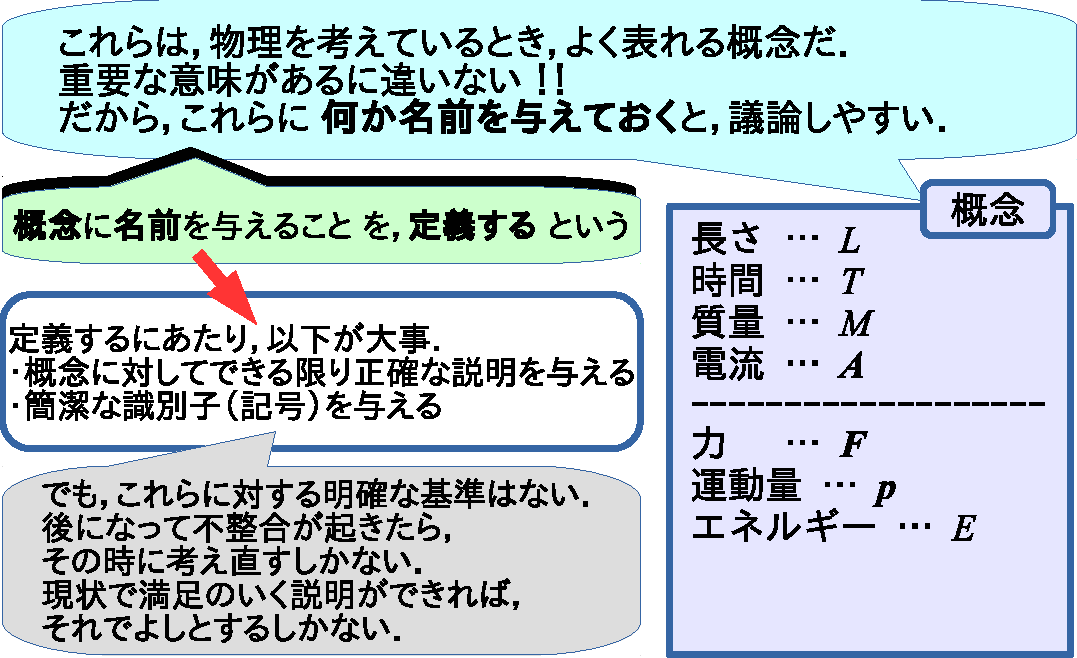
\includegraphics[keepaspectratio, width=6.5cm,height=4cm,clip]{teigi.pdf}
                            \caption{定義しよう!!}
                            \label{fig:teigi}
                        \end{center}
                    \end{figure}

                もちろん,定義した物理量が妥当でなかったと分かった場合,その定義を
                見直さなければならない.妥当でないというのは,実験事実と矛盾するこ
                とや,あるいは,全く的外れな定義等である.このようなことは,理論を
                作っていく上で必ず生じることであり,やむを得ない.

                このノートで定義される物理量は昔からその正しさが確認されているもの
                であり,従って,このノートで定義される物理量は今後も変化することが
                ないだろう
                    \footnote{
                        万が一,理論や実験技術の発展によって変更されることが余儀な
                        くされても,それは特殊な状況であるようなときに限って,定義
                        しなおされる.例えば,運動量  $\textit{\textbf{p}} = m\bv$ を
                        もつ物体はその速度が光速(光の速さ)に近いとき,相対性理論に
                        よってこの定義は見直される.詳細は,相対性理論の章を参照.
                    }.

                このノートでは「$\cdots$ と定義する」とは書かずに,「$\cdots$ という」
                と書くこともあるだろうが,これも定義のうちに入る と考えてもらいたい.

                また,物理量の定義を把握するためには演習が必要である.新しい概念が
                定義されたときは,演習書を用いてより感覚的に捉えられるようにしてお
                くとよい.先ほども書い通り,このノートで演習するようなことはない.

            \begin{memo}{「定義」の定義}
                「定義」という言葉の意味を,説明した.しかし,「定義」という語彙の
                定義をしたわけではない.単に,「定義」という難し言い回しを,噛み砕
                いて,言い直したに過ぎない.ならば,「定義」という語彙の定義は,
                どうなされるのだろうか,という疑問が浮かび上がってきたかも知れない
                    \footnote{
                        あるいは,ここの記述を読んで,疑問が提示され,不思議に思ったかもしれない.
                    }.


                しかし,実は,この疑問は意味のない疑問である.
                ゲーデールの定理などで有名な,自己言及が含まれていて,矛盾がおこるからである.
                「定義」という言葉を知らないと
                    \footnote{
                    ここでいう,「知る」という言葉は,
                    「定義」という語彙を,自分の頭で了解し,言葉で表せなくとも,感覚的に定義されている
                    ということを,念頭において使用した.
                    },
                「『定義』の定義とは何か」という疑問も起こりえない.
                一方で,「定義」という言葉の意味を知っているならば,そもそもこの疑問は起こりえない.
                    \footnote{
                        「『定義』の定義とは何か」とは何かという疑問をするためには,「定義」という言葉を
                        予め知っていないとならない.例えば,上の『定義』を一般的な語彙に拡張し,「Xの定義とは」
                        と置き換えてみるとわかりやすい.「Xの定義とは何か」と問うということは,すでに「定義」という
                        語彙を使用して疑問を投げかけているのであり,「定義」という語彙を了解した上での疑問と
                        いうことになる.そうなれば,X$=$「定義」とした時の,「『定義』の定義とは何か」という疑問を
                        投げるためには,やはり,予め「定義」という語彙を知っていないとなければならない.
                    }

                しかし,わからない.何をもって「定義」であると言えるのか.定義であるための基準とは
                何なのか.判断基準は定義と同じ意味であり,確かに,「『定義』の定義とは何か」という
                疑問と変わりなく思えるのだが,この疑問は自己矛盾を含んでいて,意味がないものである.

                私が今まで見てきた数学の解説書や参考書には,定義という言葉の意味を説明はされているものは
                あったが,定義であるための満たすべき基準が書かれたものは,見たことがない.

                どういうことだろうか.私の現在の解釈は,「定義」という語彙は名詞としてではなく,
                「定義する」という動詞として存在している,というものである.「定義する」という動詞は,
                ある語彙を,曖昧さなく
                    \footnote{
                        「曖昧」という語彙の意味も曖昧だ.ここでは,後の議論に論理的に相反する結果を
                        起こさない程度,と認識してもらいたい.
                    },
                より明確に意味づけを行う行為である,と考えるのだ.
            \end{memo}

%   %==========================================================================
%   %  Section
%   %==========================================================================
    \section{物理学の基本概念}
%       %======================================================================
%       %  SubSection
%       %======================================================================
        \subsection{物理量}
            物理的に意味のある量
                \footnote{
                    物理的に意味のある量とは,
                    「そのような量を導入することで現象がうまく説明できる」
                    という量である.
                }
            を \textbf{物理量} という.例えば,速度や加速度,重さ,長さ,時間などだ.
            運動量や力積,エネルギーや仕事量なども物理量である.実験により観測できる量
            は,すべて物理量であると思ってよい.

%       %======================================================================
%       %  SubSection
%       %======================================================================
        \subsection{物体}
            いままで,「もの」という表現を使っていたが,これからはもっとかっこよ
            く,\textbf{物体} ということにしよう.こっちのほうが,なんだか畏まっ
            てして,学問をしている感じになる.何でも難しく言えばいいということで
            はないのだけども,暗黙の了解をその言葉に含めるにはちょうどよいので
            ある.

            ここで,「物体」と表現したときに,暗黙の了解とされている性質を説明し
            よう.

            「もの」には,さまざまな性質がある.形,色,硬さ,におい等.また,そ
            の「もの」が食べ物であったなら,食感や味,風味もある.動物であれば,
            暖かさとか,おとなしいとか落ち着きがないとかなどの性格も,考えられる
            はずだ.一口に「もの」といってしまえば,こういう性質を全て考えなけれ
            ばならなくなる.けれど,これではあまりにも広い範囲の対象を相手にしな
            ければならず,一度に相手にするにはとても難しい
                \footnote{
                    難しい:不可能なことでない.「難しい」と表現されたときには,
                    原理的には可能なのであるが,実際に行うととても時間がかかる,
                    ということを意味している.例えば,「難しい問題」という表現が
                    ある.難しい問題とは,とくのに非常に時間のかかる(どれくらい
                    時間がかかるかは問題による)問題のことである.決して解けない
                    問題ではないのだ.まあ,そもそも「解けない問題」は問題ではな
                    い.だって,答えがないということがわかっているのだから(哲学
                    てきに難しい問題といわれたら,「“答え”のない問題」なのかも
                    知れないが).
                }.
            そこで,考える「もの」に制限を与えて,対象の範囲を狭くするのである.
            その制限とは,色とか,におい,味,食感,性格等は無視するということで
            ある.主に考えるのは,重さ,形,硬さである.どれに着目するかは,その
            つど異なるが,とにかく全ての性質を同時に扱うことは,難しいのでやらな
            い.

            特に,\textbf{物体} と言われたときには,「もの」の大きさと形しか考え
            ず,においとかの他の性質は全く考慮しないことを,暗に主張する.物理
            学でいう「物体」とは,日常生活で使用する言葉の“物体”とは異なる
                \footnote{
                    日常生活で使用する“物体”と同じ意味で,今まで「もの」と表現
                    していた.
                }.


%       %======================================================================
%       %  SubSection
%       %======================================================================
        \subsection{系}
            考える対象全体のことを \textbf{系} という.例えば,$N$ 個の物体の運動
            について考えるときに,「系全体」といわれたならば,それは,「$N$ 個の
            物体に関わるもの全て」ということ と同じ意味である.

            例えば,積み木が積まれている台車が運動しているとしよう.この台車がど
            のような動きをするのかを考えるとき,この積み木と台車の両方について考
            える必要がある.このときの系全体とは,「台車と積み木」である.太陽に
            対する地球の自転を考えるときの系全体とは太陽と地球のことである.より
            正確には周囲の他の惑星も系とすべきだ.要するに,今何を対象に考えてい
            るかとか,何に注目しているだとかの,そのような対象(もの)を総じて系と
            いうのだ.

%       %======================================================================
%       %  SubSection
%       %======================================================================
        \subsection{文字・数式・式変形}
            \begin{mycomment}
            物理学において,数式とは推論の道具に過ぎない.しかし,それは途方も
            なく有用な道具である.数式の持つ意味について,考える.
            \end{mycomment}

        \begin{mysmallsec}{文字}
            数式は文字で表現される.そして,文字は互いに関係付けられている.具
            体例で考える.ここに一冊の本があるとする.本には色々な性質が備わ
            っている.重さや色,紙の質,書かれている文字,匂い等,色々とある.
            物理学では,これら本のもつ諸性質のうち,特に関心があるのが,重さで
            ある.そこで,ここでは本の重さのみについて考えることにし,その他
            の性質(匂いやその記述されている内容)は全く無視してしまおう.それ
            で,本の重さについての記述をしたいのだが,どうすればよいだろう.
            なんて問うまでもなく,「重さを $W$ とおく」と表現すれば良い.「重さ
            を $W$ とおく」と表現したことにより,現実にある本の重さが,文字 $W$ で
            表現され,重さを数学的に扱うことが可能になった.視点を数式目線に変更
            して考えて見れば,文字 $W$ に重さという意味が与えられたとも考えるこ
            ともできよう.
        \end{mysmallsec}


        \begin{mysmallsec}{数と数字}
            ものの個数
                \footnote{
                    例えば,りんごの個数だとか,鉛筆の本数だとか,本の冊数だとか,
                    家の件数だとか,
                }
            や物の値段などで使われる,概念を抽象化したものを \textbf{数} という
                \footnote{
                    「スウ」と読む.「カズ」と読んでも間違いではないが,
                    数学をしている時には「スウ」と言う方が一般的.
                }.

            "数" を文字で表したものを \textbf{数字} という.同じ数に対して,
            いろいろな字が割り当てられていて,例えば,以下はすべて同じ数を示す文字である:
                \begin{equation*}
                    4 \,, \qquad \mbox{四} \,, \qquad \IV
                \end{equation*}
            数を表す文字は複数種類あり,どれを使っても良い.
            一般的に,\textbf{アラビア数字} と呼ばれる以下の数字が便利であり,多く使用される:
                \begin{equation*}
                    0 \, , \quad  1 \, , \quad  2 \, , \quad  3 \, , \quad
                    4 \, , \quad  5 \, , \quad  6 \, , \quad  \ldots
                \end{equation*}
            数式内の数字はアラビア数字を使う.文章内の数字はアラビア数字も使用するが,
            \textbf{漢数字} も使用する.漢数字とは,以下のような数字である:
                \begin{equation*}
                    \mbox{一}\, , \quad \mbox{二} \, , \quad \mbox{三}   \, , \quad \mbox{四} \, , \quad
                    \mbox{五}\, , \quad \mbox{六} \, , \quad \ldots
                \end{equation*}
            他にも,\textbf{ギリシア数字} ($\I$,$\II$,$\III$,$\IV$,$V$,$\VI$,$\ldots$) も数字だし,
            「正」の字を使って数えるときの途中段階の文字(記号?)も数字である.まあ,色々とあるが,
            物理学を勉強していく上では,上記のような常識的な範囲の数字の扱い方ができていれば十分である.
        \end{mysmallsec}

        \begin{mysmallsec}{変数}
            具体的な数($1,\,2,\,3,\,\ldots$)ではなく,"全ての数に対しての記述"をしたい場合がある
                \footnote{
                    数全般の性質を表したい場合は,具体的な数字を使って表現するわけににはいかない.
                    具体的な数字を使ってしまうと,その数にしか成り立たない記述になってしまう.
                }.
            そういった場合,\textbf{変数} という考え方を使う.
            全ての数に当てはまるということは,どんな数にも変わり得るということ.
            変数を表す記号は,様々である.
            中学や高校数学では,$x$ や $y$ や $z$ が使われる.また,$\theta$ や $\phi$ などの
            ギリシャ文字を使うことも多い.

            もっと高度な数学になると,
            変数が無限に多く欲しい場合があり.その場合は,アルファベットでは対応できない.だから,
            以下のように,アルファベットの右下や右上にアラビア数字を添えて,
                \begin{equation*}
                    {x}_{1} , \quad {x}_{2} , \quad {x}_{3} , \quad \ldots
                \end{equation*}
            と言った感じで,無限に変数を増産できる
                \footnote{
                    あるいは,
                    \begin{equation*}
                        {x}^{1} , \quad {x}^{2} , \quad {x}^{3} , \quad \ldots
                    \end{equation*}
                    でもよい.添字は右上でも右下でもどちらでも構わない.今のところは,
                    添字の位置には特に意味を与えていないが,後々(相対性理論を勉強する段階)では,
                    この添字の位置に意味を与えるので,注意が必要だ.
                }.
            添字は無限に増やせるからだ.だが,これでも,
            変数を無限に列挙することなどはできない.そこで,「$i$ は任意の自然数であるとする」という
            文言を添えて,
                \begin{equation*}
                    {x}_{i}
                \end{equation*}
            の一文字で済ますことが可能である
                \footnote{
                    $i$ には 1でも2でも99でも何でもよく,とにかく全ての自然数が順に与えられて,
                    整列させられているイメージを持って欲しい.そのイメージを具体的に書くと,${x}_{i}$ と
                    書かれた場合,
                    \begin{equation*}
                        {x}_{i}
                        \leftrightarrow
                        \left( 1,\,2,\,3,\,4,\,5,\,6,\,\ldots,\,i,\,\ldots,\,\infty \right)
                    \end{equation*}
                    ということである.$\leftrightarrow$ はその左側と右側で同じ意味を持つことを示す
                    ものである.

                    また,ここで,\textbf{無限} について定義せずに使用しているが,普段の
                    生活の意味の無限として捉えていて問題ない.無限を真面目に考え始めると,
                    深みにハマってしまい,議論が終わらなっくなってしまう.無限についての理解は
                    この程度で十分であろう:
                        \begin{equation*}
                            \mbox{無限大 とは,全ての数よりも大きい ということである.}
                        \end{equation*}
                        \begin{equation*}
                            \mbox{無限小 とは,全ての数よりも小さい ということである.}
                        \end{equation*}
                    "ということ" と表現したのには意味がある."という数" と書いていしまうと,
                    自己言及して矛盾になってしまう,「"全ての数" よりも大きい"数"」なんて
                    文は矛盾.だって,"全ての数"って言っているんだから,これよりも大きい数って,
                    全ての数以外の数だということになって,つまり,「"全ての数"以外の数」があることになる.
                    「"全ての数"以外の数」なんてものは矛盾.要するに,無限を数として扱ってはならない
                    ということである.
                }.

            変数の例を上げると,$f(x)=ax+b$ や $g(\theta)=\sin\theta$ と書かれた時の,
            $x$ と $\theta$ がそれに当たる.この場合の $x$ と $\theta$ は関数の定義域の全ての
            実数値を取りうることを意味付けられている.
        \end{mysmallsec}

        \begin{mysmallsec}{定数}
            ある特定の数(固定された値)であるが,それが特別な数ではない場合,これを \textbf{定数} という.
            読み方は,「ジョウスウ」または「テイスウ」である
                \footnote{
                    普通は「テイスウ」と読む.年齢を重ねた人が「ジョウスウ」と読む,という勝手なイメージがある.
                }.

            低すを表す記号として,アルファベットの最初の文字 $a$,$b$,$c$,$d$ などが使われる.大文字の $A$,$B$,
            $C$ が使われることも多い.変数に比べると,様々な文字が定数を表す記号として使われる傾向にある.
            ただ,教科書にはその都度,それが定数であるか変数であるかを説明しているので,どっちかわからずに混乱
            することはないだろう.

            先にも上げた例だと,$f(x)=ax+b$ とした場合の,$a$ や $b$ が定数である.
        \end{mysmallsec}

        \begin{mysmallsec}{整数(自然数,負の数),有理数}
            このノートでは,$0$ を含めた以下を \textbf{自然数} とよぶ:
                \begin{equation*}
                    0,\,1,\,2,\,3,\,4,\,5,\,6,\,7,\ldots
                \end{equation*}

            負の数とは,ある定数 $A$ に対して $A+x=0$ となるような $x$ のことをいい,$x:=-A$ と
            書く慣習がある.例えば,$A=1$ の時は,$x=-A=-1$ だし,$A=100$ だったら,$x=-100$ である.

            自然数と負の数を大きさ順に具体的に並べてみると,以下のようになる(右にあるほど大きい):
                \begin{equation*}
                    -4,\,-3,\,-2,\,-1,\,0,\,1,\,2,\,3,\,4\ldots
                \end{equation*}
            記号 $-$ のことを,\textbf{マイナス} とう.「負の数」という新たらしい数が作られたことで,
            今まであった0以外の自然数のことを \textbf{正の数} とよぶこともあり,記号は $+$ を使う.
            記号 $+$ は\textbf{プラス} という.「マイナス」と「プラス」は英語のplusとminusであり,
            "正"と"負"はこの英語に対して割り当てられた日本語語彙である.
            自然数と負の数を総称して,\textbf{整数} という.

            整数を2つ用意して(用意した2つが同じ整数でもいい)以下のように表した時,
            これを \textbf{有理数} という:
                \begin{equation*}
                    \frac{1}{2} \;,\;\; \frac{-9}{123} \;,\;\; \quad \frac{4}{-5} \;,\;\; \quad \frac{-9}{-177}
                \end{equation*}
            上記のように,真ん中に短い線を引いて2つの数を上下に記述した有理数の表現手法を \textbf{分数} という
                \footnote{
                    分数を一行で記述したい場合もある.こういう時は,1/2 とか -9/123 などと書く.
                    記号"/"を数の間に入れて分数を表現するのである.
                }.
            0 は下に書くことはできない
                \footnote{
                    0を下に書くと,四則演算で論理的に不整合な計算ができてしまい,体系に矛盾が生じる.
                    例えば,$\frac{1}{0}$ という数を書いてみる.
                    どんな数でも0をかければ,0になるので(これは0元の公理で,有無を言わずに認めることである),
                    $\frac{1}{0} \times 0 = 0$ となるのだが,この式の左辺は $\frac{1}{0} \times 0 = 1$ とも計算できる.
                    すると,$1=0$ となって論理的に不整合(矛盾)になる.矛盾が生じた理由は,
                    そもそも $\frac{1}{0}$ という数が存在すると仮定したからである.要するに矛盾を起こさないためには,
                    $\frac{1}{0}$ というような分母に0を置くような有理数(分数)を考えてはいけないということだ.
                }.
            また,上の数のことを \textbf{分子} といい,
            下の数のことを \textbf{分母} という.分子と分母の両方が負の数の時は,
            その両方のマイナスを取り去っても同じ分数としてあつかう:
                \begin{equation*}
                    \frac{-9}{-177} = \frac{9}{177}.
                \end{equation*}
            分母と分子のどちらか一方のみが負の数の場合は,負の分数として扱い,マイナス記号を
            分数の左真ん中へ移動させて書く:
                \begin{equation*}
                    \frac{-9}{123} = \frac{9}{-123} = -\frac{9}{123}.
                \end{equation*}

            分数の具体的なイメージは,割合だろう.全体の数を分母とし,分子には今注目している部分の数を書く.
            こうしてあらわされた分数は,注目している箇所は全体のどれくらいかを示す量となる
                \footnote{
                    あくまでも,分数を現実と対比させたい場合の例である.
                    数学では,このような具体的なイメージから発展させ,より抽象化される.
                    この例にとらわれると,マイナスの数が分母に書かれたときに,全体の数がマイナスになるが
                    どういうことだろうかと,無駄な考えに陥るかもしれない.数は現実の世界から必要に迫られて
                    人間が生み出したものであるが,数学ではそれを抽象化して数の性質を探求する学問である.
                    現実との具体的な対比に悩むのはナンセンスだ(物理学では大事なことだが).
                }.
        \end{mysmallsec}

        \begin{mysmallsec}{等号,不等号}
            2つの数を比較して,どちらが大きいか(あるいは小さいか)を文字で書きたいことがある.
            その場合,2つの数 $a,\,b$ を比較して,$a$ が $b$ よりも大きい場合は $a>b$ または $b<a$と書く.
            $b$ の方が $a$ よりも大きい場合は $a<b$ または $b>a$ とかく.$a$ と $b$ が
            等しい場合は $a=b$ とかく.記号にも名前があり,$=$ を \textbf{等号} といい,
            $<,\,>$ の2つを \textbf{不等号} という.不等号が2種類あると思われるかもしれないが,
            向きをどうするかの($a$ と $b$ の並べ方)違いであり,実際上,1種類記号である.
        \end{mysmallsec}

        \begin{mysmallsec}{演算,演算器号}
            演算には,「加算」と「乗算」がある.加算は記号 $+$ で表され,乗算は記号 $*$ で表される.
            加算と乗算はどういった計算かを一般的に示すことはできないので,以下に具体例を書くに留める.
            \begin{equation*}
                \mbox{加算: } 1+1=2 ,\quad 12=6+3+2+1
            \end{equation*}
            \begin{equation*}
                \mbox{乗算: } 1*1=1 ,\quad 36=6*3*2*1
            \end{equation*}

            加算と乗算以外にも,減算と除算があると思われるかもしれないが,減算と除算は加算と乗算の一部
            として含めることができる.減算の場合には,加算に対して負の数を導入することで,実現できる.
            つまり,
            \begin{equation*}
                \mbox{減算: } 1-1=1+(-1) , \quad 4=6+(-3)+2+(-1)
            \end{equation*}
            のように,減算ではなく負の数との加算だと解釈すれば,減算は加算のとみなせる.
            除算の場合には少し強引に聞こえるかもしれないが,分子を1とする分数と整数の除算,つまり,
            \begin{equation*}
                \mbox{除算: } 1 \divisionsymbol 2=\frac{1}{2}=1*\frac{1}{2} ,\quad 5 \divisionsymbol 6=\frac{5}{6}=5*\frac{1}{5}
            \end{equation*}
            と考えることで,除算を乗算の一部とみなせる.

        \end{mysmallsec}

        \begin{mysmallsec}{数式}
            世の中には非常に多くの本がある.本だけではない.鉛筆,ボー
            ルペン,コンパス,定規,机の上にあるものだけ上げても,非常に多くの
            ものが存在している.話を簡単にするために,机の上には,鉛筆と消しゴ
            ムと本がそれぞれ一つずつ存在し,これ以外のものは置いていないとしよ
            う.やはりこの3つのモノにも重さがあり,それを $W_{\mbox{鉛筆}}$,$W_{\mbox{消しゴム}}$,
            $W_{\mbox{本}}$ と表現することにしよう.これら3つの重さについて関心がある
            のは,それらの「関係」だろう.「関係」といったのは,どれが最
            も重いかとか,軽いかといったことである.この「関係」を数学的に扱
            うには,数式を使うと非常に簡単に表現できる.例えば,鉛筆の重さと消
            しゴムの重さが全く同じ時には,
                \begin{equation*}
                    W_{\mbox{鉛筆}} = W_{\mbox{消しゴム}}
                \end{equation*}
            と表現できることは,周知のことであると思う
                \footnote{
                    哲学的な疑問はここでは考えないことにしよう.数式は文字の羅
                    列である.ここで言うと,
                        \begin{center}
                            $W$,$=$,鉛,筆,消,し,ゴ,ム
                        \end{center}
                    という記号の羅列と捉えられる.文字の羅列になぜ意味を感じるの
                    か.うーん,難しい.とりあえず,この疑問は保留にしておこう.
                }.
            数式とは,文字と文字の「関係」を表現できるものである.
        \end{mysmallsec}

        \begin{mysmallsec}{式変形}
                        文字と数式には意味があり,特に物理学において文字と数式は,現実
            世界と強く結びついている.現実に起きている現象を数式で表すことが,物
            理学のひとつの方法なのだから.では,「式変形」に意味はあるのだろうか.
            結論から言えば,「式変形」それ自体にはなんの意味もない.単に,数学
            的に定義された文字の操作を行っているに過ぎない.にもかかわらず,「式
            変形」は非常に重要なのである.実際,式変形を行うことにより,いろいろ
            と推論を行うことができるし,また,それによって物理学が発展しているの
            である.意味が無いのに重要であるとは,いったいどういう事なのか.答え
            は,式変形を行うことにより,論理的必然性を確かめることができることに
            ある.何らかの意味をもった数式に式変形を施すことで,別の意味の数式を導出す
            る.これにより,正しい推論を行うことができるのである.世の中には論理
            的に矛盾したことは起こりえないから
                \footnote{
                    そもそも,論理的に矛盾していることを想像することもできない.
                    「ここに本があり,かつ,その同じ場所に本がない」という状況
                    を思い描くことが可能だろうか.
                },
            論理立てて考えることで,間違った結論を出すことは,ぐっと少なくなるは
            ずである.式変形を行うということは,論理的推論を行うということであり,
            そうして得た結論は,論理的に必然性を持つものであり,実験して確かめる
            価値は十分にあると言える.ちなみに,ここで言う必然性とは,物理学的に
            考えて必然ということであり,論理的に厳密に必然であることをいうのでは
            ない.物理学における論理的推論とは,「物理学的に考えてもっともらしい仮定」
            をもとにするため,この点において多少の厳密性が犠牲にされている.
        \end{mysmallsec}


        \begin{memo}{$a+b=b+a$ ?}
            $4+3=7$という足し算を考えよう.当然,$3$と$4$を入れ替えて書いて,$3+4=7$と書いても同じ.
            また,等号の右と左を入れ替えて,$7=4+3$あるいは,$7=3+4$としても,等式は成り立つ.
            本当にそうだろうか.$3+4$は$4+3$に同じなのか.実際のところ,違うだろう.
            3つのイチゴと4つのリンゴは,4つのイチゴと3つのリンゴとはことなる.
            確かに,個数だけに着目すれば$3+4=4+3$になるが,イチゴとリンゴの個数としての数字であると
            考える場合には,この等式は成り立たない.
            また,$3+4=7$という式を言葉にすると「3足す4は7である」と表現するのが自然であり,
            他方,$7=3+4$は同じように言い表すと「7は3足す4である」となる.両者の意味は全く違う.
            「7は3足す4である」は間違ってはいないが,決めつけているような表現であり,抵抗を感じる
                \footnote{
                    $7=5+2$でも,$7=1+6$でも,$7=10-3$でもよいのである.
                }.
            $3+4$も$4+3$も$5+2$も$10-3$も数式として考えれば,計算結果はすべて等しく,7である
                \footnote{
                    $3+4$という計算結果と,$4+3$という計算結果が等しく,両者とも互いに置き換えることが
                    できるということ.
                }.
            式計算する場合に,数や式に意味を考えてしまうと,余計なことを考え出してしまう(「$4+3$と$3+4$は同じか」とか).
            式計算時には数を抽象化してとらえなければならない
                \footnote{
                    きっとここら辺に数学の素晴らしさがあるのだろう.
                    こういう抽象化が興味深い体系的の数学を構成する基礎になっていくのだと感じる.
                }.

            一方で,物理学では単位という概念がある
                \footnote{
                    長さ[m],時間[s],質量[kg],電流[A]など.
                }.
            物理学で扱う数字には意味が込められており,計算時に単位を意識する必要がある.
            単位が違う数字の足し算は認められていない
                \footnote{
                    長さ1[m] + 質量1[kg] という計算は全く意味不明だ.
                }.
            掛け算は認められている
                \footnote{
                    だからこそ,新しい概念を作ることができる.
                    エネルギーの単位[J]は,力1[N]と長さ1[m]の積として定義されている.
                    ($[\mbox{J}] := [\mbox{N} \cdot \mbox{m}].$)
                }.
            単位は数学にはない概念である
                \footnote{
                    ここにも,科学と数学の違いが表れている.
                }.
            物理学で数式を扱う場合,数学と全く同じように扱ってしまうと,
            単位の違う数字の足し算をしてしまうという誤りをしがちである.
        \end{memo}
